% Options for packages loaded elsewhere
\PassOptionsToPackage{unicode}{hyperref}
\PassOptionsToPackage{hyphens}{url}
%
\documentclass[
  man, donotrepeattitle,mask,floatsintext]{apa6}
\usepackage{amsmath,amssymb}
\usepackage{lmodern}
\usepackage{iftex}
\ifPDFTeX
  \usepackage[T1]{fontenc}
  \usepackage[utf8]{inputenc}
  \usepackage{textcomp} % provide euro and other symbols
\else % if luatex or xetex
  \usepackage{unicode-math}
  \defaultfontfeatures{Scale=MatchLowercase}
  \defaultfontfeatures[\rmfamily]{Ligatures=TeX,Scale=1}
\fi
% Use upquote if available, for straight quotes in verbatim environments
\IfFileExists{upquote.sty}{\usepackage{upquote}}{}
\IfFileExists{microtype.sty}{% use microtype if available
  \usepackage[]{microtype}
  \UseMicrotypeSet[protrusion]{basicmath} % disable protrusion for tt fonts
}{}
\makeatletter
\@ifundefined{KOMAClassName}{% if non-KOMA class
  \IfFileExists{parskip.sty}{%
    \usepackage{parskip}
  }{% else
    \setlength{\parindent}{0pt}
    \setlength{\parskip}{6pt plus 2pt minus 1pt}}
}{% if KOMA class
  \KOMAoptions{parskip=half}}
\makeatother
\usepackage{xcolor}
\usepackage{graphicx}
\makeatletter
\def\maxwidth{\ifdim\Gin@nat@width>\linewidth\linewidth\else\Gin@nat@width\fi}
\def\maxheight{\ifdim\Gin@nat@height>\textheight\textheight\else\Gin@nat@height\fi}
\makeatother
% Scale images if necessary, so that they will not overflow the page
% margins by default, and it is still possible to overwrite the defaults
% using explicit options in \includegraphics[width, height, ...]{}
\setkeys{Gin}{width=\maxwidth,height=\maxheight,keepaspectratio}
% Set default figure placement to htbp
\makeatletter
\def\fps@figure{htbp}
\makeatother
\setlength{\emergencystretch}{3em} % prevent overfull lines
\providecommand{\tightlist}{%
  \setlength{\itemsep}{0pt}\setlength{\parskip}{0pt}}
\setcounter{secnumdepth}{-\maxdimen} % remove section numbering
% Make \paragraph and \subparagraph free-standing
\ifx\paragraph\undefined\else
  \let\oldparagraph\paragraph
  \renewcommand{\paragraph}[1]{\oldparagraph{#1}\mbox{}}
\fi
\ifx\subparagraph\undefined\else
  \let\oldsubparagraph\subparagraph
  \renewcommand{\subparagraph}[1]{\oldsubparagraph{#1}\mbox{}}
\fi
\newlength{\cslhangindent}
\setlength{\cslhangindent}{1.5em}
\newlength{\csllabelwidth}
\setlength{\csllabelwidth}{3em}
\newlength{\cslentryspacingunit} % times entry-spacing
\setlength{\cslentryspacingunit}{\parskip}
\newenvironment{CSLReferences}[2] % #1 hanging-ident, #2 entry spacing
 {% don't indent paragraphs
  \setlength{\parindent}{0pt}
  % turn on hanging indent if param 1 is 1
  \ifodd #1
  \let\oldpar\par
  \def\par{\hangindent=\cslhangindent\oldpar}
  \fi
  % set entry spacing
  \setlength{\parskip}{#2\cslentryspacingunit}
 }%
 {}
\usepackage{calc}
\newcommand{\CSLBlock}[1]{#1\hfill\break}
\newcommand{\CSLLeftMargin}[1]{\parbox[t]{\csllabelwidth}{#1}}
\newcommand{\CSLRightInline}[1]{\parbox[t]{\linewidth - \csllabelwidth}{#1}\break}
\newcommand{\CSLIndent}[1]{\hspace{\cslhangindent}#1}
\ifLuaTeX
\usepackage[bidi=basic]{babel}
\else
\usepackage[bidi=default]{babel}
\fi
\babelprovide[main,import]{english}
% get rid of language-specific shorthands (see #6817):
\let\LanguageShortHands\languageshorthands
\def\languageshorthands#1{}
% Manuscript styling
\usepackage{upgreek}
\captionsetup{font=singlespacing,justification=justified}

% Table formatting
\usepackage{longtable}
\usepackage{lscape}
% \usepackage[counterclockwise]{rotating}   % Landscape page setup for large tables
\usepackage{multirow}		% Table styling
\usepackage{tabularx}		% Control Column width
\usepackage[flushleft]{threeparttable}	% Allows for three part tables with a specified notes section
\usepackage{threeparttablex}            % Lets threeparttable work with longtable

% Create new environments so endfloat can handle them
% \newenvironment{ltable}
%   {\begin{landscape}\centering\begin{threeparttable}}
%   {\end{threeparttable}\end{landscape}}
\newenvironment{lltable}{\begin{landscape}\centering\begin{ThreePartTable}}{\end{ThreePartTable}\end{landscape}}

% Enables adjusting longtable caption width to table width
% Solution found at http://golatex.de/longtable-mit-caption-so-breit-wie-die-tabelle-t15767.html
\makeatletter
\newcommand\LastLTentrywidth{1em}
\newlength\longtablewidth
\setlength{\longtablewidth}{1in}
\newcommand{\getlongtablewidth}{\begingroup \ifcsname LT@\roman{LT@tables}\endcsname \global\longtablewidth=0pt \renewcommand{\LT@entry}[2]{\global\advance\longtablewidth by ##2\relax\gdef\LastLTentrywidth{##2}}\@nameuse{LT@\roman{LT@tables}} \fi \endgroup}

% \setlength{\parindent}{0.5in}
% \setlength{\parskip}{0pt plus 0pt minus 0pt}

% Overwrite redefinition of paragraph and subparagraph by the default LaTeX template
% See https://github.com/crsh/papaja/issues/292
\makeatletter
\renewcommand{\paragraph}{\@startsection{paragraph}{4}{\parindent}%
  {0\baselineskip \@plus 0.2ex \@minus 0.2ex}%
  {-1em}%
  {\normalfont\normalsize\bfseries\itshape\typesectitle}}

\renewcommand{\subparagraph}[1]{\@startsection{subparagraph}{5}{1em}%
  {0\baselineskip \@plus 0.2ex \@minus 0.2ex}%
  {-\z@\relax}%
  {\normalfont\normalsize\itshape\hspace{\parindent}{#1}\textit{\addperi}}{\relax}}
\makeatother

% \usepackage{etoolbox}
\makeatletter
\patchcmd{\HyOrg@maketitle}
  {\section{\normalfont\normalsize\abstractname}}
  {\section*{\normalfont\normalsize\abstractname}}
  {}{\typeout{Failed to patch abstract.}}
\patchcmd{\HyOrg@maketitle}
  {\section{\protect\normalfont{\@title}}}
  {\section*{\protect\normalfont{\@title}}}
  {}{\typeout{Failed to patch title.}}
\makeatother

\usepackage{xpatch}
\makeatletter
\xapptocmd\appendix
  {\xapptocmd\section
    {\addcontentsline{toc}{section}{\appendixname\ifoneappendix\else~\theappendix\fi\\: #1}}
    {}{\InnerPatchFailed}%
  }
{}{\PatchFailed}
\keywords{social norms; descriptive norms; injunctive norms; longitudinal; COVID-19; mask wearing; cooperation\newline\indent Word count: 4521 words}
\usepackage{lineno}

\linenumbers
\usepackage{csquotes}
\usepackage{array}
\usepackage{caption}
\usepackage{graphicx}
\usepackage{siunitx}
\usepackage[normalem]{ulem}
\usepackage{colortbl}
\usepackage{multirow}
\usepackage{hhline}
\usepackage{calc}
\usepackage{tabularx}
\usepackage{threeparttable}
\usepackage{wrapfig}
\usepackage{adjustbox}
\usepackage{hyperref}
\usepackage{setspace}
\raggedbottom
\AtBeginEnvironment{tabular}{\singlespacing}
\AtBeginEnvironment{lltable}{\singlespacing}
\AtBeginEnvironment{tablenotes}{\doublespacing}
\captionsetup[table]{font={stretch=1,small}}
\captionsetup[figure]{font={stretch=1,small}}
\ifLuaTeX
  \usepackage{selnolig}  % disable illegal ligatures
\fi
\IfFileExists{bookmark.sty}{\usepackage{bookmark}}{\usepackage{hyperref}}
\IfFileExists{xurl.sty}{\usepackage{xurl}}{} % add URL line breaks if available
\urlstyle{same} % disable monospaced font for URLs
\hypersetup{
  pdftitle={Descriptive, not injunctive, social norms caused increases in mask wearing during the COVID-19 pandemic},
  pdflang={en-EN},
  pdfkeywords={social norms; descriptive norms; injunctive norms; longitudinal; COVID-19; mask wearing; cooperation},
  hidelinks,
  pdfcreator={LaTeX via pandoc}}

\title{Descriptive, not injunctive, social norms caused increases in mask wearing during the COVID-19 pandemic}
\author{Samantha L. Heiman\textsuperscript{*,1}, Scott Claessens\textsuperscript{*,2}, Jessica D. Ayers\textsuperscript{3}, Diego Guevara Beltrán\textsuperscript{4}, Andrew Van Horn\textsuperscript{5,6}, Edward R. Hirt\textsuperscript{1}, Athena Aktipis\textsuperscript{†,4}, \& Peter M. Todd\textsuperscript{†,1,7}}
\date{}


\shorttitle{Norms and mask wearing}

\affiliation{\vspace{0.5cm}\textsuperscript{1} \footnotesize Department of Psychological and Brain Sciences, Indiana University Bloomington, United States\\\textsuperscript{2} \footnotesize School of Psychology, University of Auckland, New Zealand\\\textsuperscript{3} \footnotesize Department of Psychological Science, Boise State University, United States\\\textsuperscript{4} \footnotesize Department of Psychology, Arizona State University, United States\\\textsuperscript{5} \footnotesize Department of Physics, Case Western Reserve University, United States\\\textsuperscript{6} \footnotesize Department of Art History, Case Western Reserve University, United States\\\textsuperscript{7} \footnotesize Cognitive Science Program, Indiana University Bloomington, United States}

\note{

\footnotesize 

\raggedright

\mbox{* indicates shared first authorship, † indicates shared senior authorship}

\par

Correspondence concerning this article should be addressed to Samantha L. Heiman, 1101 E 10th St, Bloomington, IN 47405, United States. E-mail: \href{mailto:slheiman@iu.edu}{\nolinkurl{slheiman@iu.edu}}

\par

This study was funded by the Interdisciplinary Cooperation Initiative, ASU President's Office, the Cooperation Science Network, the Institute for Mental Health Research, the University of New Mexico, the Indiana University College of Arts \& Sciences, the Rutgers University Center for Human Evolutionary Studies, the Charles Koch Foundation, and the John Templeton Foundation.

\par

This working paper has not yet been peer-reviewed.

}

\abstract{%
Human sociality is governed by two types of social norms: injunctive norms, which prescribe what people \emph{ought} to do, and descriptive norms, which reflect what people \emph{actually} do. The process by which these norms emerge and their causal influences on cooperative behavior over time are not well understood. Here, we study these questions through social norms influencing mask wearing during the COVID-19 pandemic. Leveraging two years of data from the United States (18 time points; \emph{n} = 915), we tracked mask wearing and perceived injunctive and descriptive mask wearing norms as the pandemic unfolded. Longitudinal trends suggested that norms and behavior were tightly coupled, changing quickly in response to public health recommendations. In addition, longitudinal modelling revealed that descriptive norms, not injunctive norms, caused future increases in mask wearing. During uncertain times, cooperative behavior is driven by what others are actually doing, rather than what others think ought to be done.
}



\begin{document}
\maketitle

\hypertarget{statement-of-relevance}{%
\section{\texorpdfstring{\normalfont Statement of Relevance}{Statement of Relevance}}\label{statement-of-relevance}}

Social norms have been identified as important drivers of human cooperation, but the emergence of social norms within populations and their subsequent effects on cooperative behavior are not well understood. Here, we use mask wearing during the COVID-19 pandemic as a real-world setting in which to study the emergence of social norms. Over two years in the United States, we find that social norms and mask wearing are tightly coupled and change quickly in response to public health recommendations. Moreover, longitudinal modeling suggests that mask wearing is causally preceded by perceptions of descriptive norms (i.e.~what people \emph{are} doing) but not injunctive norms (i.e.~what people \emph{ought} to be doing). These findings show that visible community adherence is an important driver of mask wearing, suggesting potential avenues for behavior change in future global pandemics.

\newpage

\begin{center}Descriptive, not injunctive, social norms caused increases in mask wearing during the COVID-19 pandemic\end{center}

Social norms are a key aspect of human sociality (Bicchieri \& Xiao, 2009; Cialdini et al., 1991; Fehr \& Schurtenberger, 2018). Broadly, social norms are defined as commonly known behavioral guidelines enforced by groups of people (Legros \& Cislaghi, 2020). By coordinating the behavior of many individuals, social norms enable human groups to cooperate in the face of group-wide challenges and threats, such as resource scarcity, natural disasters, and infectious diseases (Roos et al., 2015). Social norms are thus hypothesized to have played a key role in the evolution of large-scale cooperation in humans (Henrich, 2015).

Previous research has distinguished between two types of social norms: injunctive norms and descriptive norms (Bicchieri \& Xiao, 2009; Cialdini et al., 1991; Deutsch \& Gerard, 1955). Injunctive norms indicate what others tend to approve or disapprove of and often involve social sanctions if violated. By contrast, descriptive norms simply describe what most people are doing in a given situation, but carry no prescriptive information \emph{per se}. According to the focus theory of normative conduct (Cialdini et al., 1991), these two kinds of social norms often align, but they can also be in conflict with one another and differentially affect behavior depending on which norm is more salient. For example, there may be an injunctive norm that cleaning up litter at a picnic site is the right thing to do: one \emph{ought} to behave this way. However, if an individual observes that most people are leaving their litter behind at the site, they may instead follow the descriptive norm and litter themselves.

Despite decades of research on injunctive and descriptive norms (Cialdini et al., 1991; Cialdini \& Jacobson, 2021; Schultz et al., 2007), open questions remain regarding the emergence and causal influence of social norms (Legros \& Cislaghi, 2020; van Kleef et al., 2019). First, how do injunctive and descriptive norms emerge over time within a population? Second, how do evolving injunctive and descriptive norms causally influence behavior over time?

Research has investigated how social norms emerge in a population over time. In the long term, cultural evolutionary models show that injunctive social norms can be vertically transmitted across generations by imitation or teaching, or horizontally diffused from neighboring populations (Henrich, 2015). However, less is known about how social norms arise endogenously within populations in the short term. Recent work in behavioral economics suggests that social norms of public good provisioning develop in tandem with cooperative behavior through repeated interactions (Titlestad et al., 2019). But it remains unclear whether these findings generalize beyond the laboratory to real human populations.

With regards to normative influences on behavior, studies have demonstrated positive effects of descriptive norms on a variety of cooperative behaviors, including recycling (Nigbur et al., 2010), paying taxes (Larkin et al., 2018), and sustainably reusing towels in hotels (Goldstein et al., 2008). However, these studies have two main limitations. First, studies have not accounted for other potential non-social explanations for behavior, such as perceptions of the effectiveness of the behavior and personal beliefs that one should behave in a certain way. These non-social beliefs, labeled ``factual beliefs'' and ``personal normative beliefs'' (Bicchieri et al., 2014), often correlate with descriptive and injunctive norms, but they are fundamentally different because they can cause behavior separately from social expectations about what others do or think should be done. For example, willingness to recycle might be driven by perceptions that recycling has a positive impact on the environment and/or personal beliefs that recycling is the right thing to do, even if social norms actively discourage recycling (e.g., recycling is not a common behavior). It is thus important to control for non-social beliefs in studies of social norms. Second, studies have tended to follow cross-sectional experimental designs. However, social norms are not static: they change dynamically over time through processes of deliberation and interaction (Smith et al., 2015). An alternative but underutilized method of assessing causality between social norms and cooperative behavior, while retaining ecological validity, is to follow these variables over time amidst a real, unfolding social dilemma.

To understand how social norms emerge over time and shape cooperative behavior in a non-experimental setting, we focus on mask wearing in the United States during the COVID-19 pandemic. In April 2020, one month after the World Health Organization declared COVID-19 a global pandemic, mask wearing was officially recommended by the Centers for Disease Control and Prevention (CDC) to minimize the spread of the disease (Centers for Disease Control and Prevention, 2022). Mask wearing has individual benefits, but the CDC also emphasized the collective benefits in reducing disease spread (Centers for Disease Control and Prevention, 2020). Indeed, mask wearing posed a social dilemma to many individuals, in that it imposed personal costs (e.g., difficulty breathing, disrupted social interaction) for the benefit of the community (e.g., ``flattening the curve'' to protect at-risk individuals). Thus, the development of mask wearing during the COVID-19 pandemic enables us to study the emergence of social norms and their causal effects on cooperative behavior over a short timescale within a single population.

Recent research has found positive relationships between social norms and protective COVID-19 behaviors. In the United States, one study found that perceptions of injunctive norms positively predicted intentions to stay at home to minimize exposure (Macy et al., 2021), and another study found that experimentally-induced descriptive norms increased mask wearing intentions (Bokemper et al., 2021). In Germany, a two-wave study found that perceptions of descriptive norms positively predicted future protective behaviors, such as physical distancing (Rudert \& Janke, 2021). These studies are telling, but since they are cross-sectional or only minimally longitudinal, they do not have the temporal granularity to capture fluctuating changes in norm strength and adherence across the pandemic. Furthermore, several of the studies do not control for political ideology, which is important to account for since COVID-19 was highly politicized in the United States (Baxter-King et al., 2022).

Here, we use two years of data from a representative sample of adults in the United States (18 time points; \emph{n} = 916) to track the development of descriptive and injunctive mask wearing norms and mask wearing behavior over the course of the COVID-19 pandemic. Participants reported their frequency of mask wearing during in-person interactions, as well as their perceptions of descriptive and injunctive mask wearing norms. We also asked participants about their non-social mask wearing beliefs and political ideology, and controlled for these factors. We used these longitudinal data to answer two main research questions in a specific real-world context. First, how do descriptive and injunctive mask wearing norms emerge over time? Second, how do descriptive and injunctive mask wearing norms causally influence mask wearing?

\hypertarget{materials-and-methods}{%
\section{Materials and Methods}\label{materials-and-methods}}

\hypertarget{ethical-approval}{%
\subsection{Ethical approval}\label{ethical-approval}}

This project was granted exemption from the Institutional Review Board of Arizona State University (STUDY00011678). All participants in this study provided informed consent.

\hypertarget{participants-and-sampling}{%
\subsection{Participants and sampling}\label{participants-and-sampling}}

Using the platform Prolific (\url{https://www.prolific.co/}), we distributed surveys to a representative sample of adults from the United States (\emph{n} = 915, \emph{M}\textsubscript{age} = 46 years, 75\% White, 52\% Women; see Supplementary Figure \ref{fig:plotUSMap} for geographic distribution). From September 2020 to October 2022, we asked participants to complete regular surveys of COVID-19 related attitudes and behaviors. This resulted in 18 unique time points of data collection during the pandemic. The first 12 time points were distributed monthly, while the remaining six time points were distributed every two months. Of the initial 915 participants, 634 returned to complete the survey at Time 2, while 347 participants continued through to Time 18 (see Supplementary Figure \ref{fig:plotAttrition} for attrition rates across all time points).

\hypertarget{measures}{%
\subsection{Measures}\label{measures}}

\hypertarget{self-reported-mask-wearing}{%
\subsubsection{Self-reported mask wearing}\label{self-reported-mask-wearing}}

At every time point, participants were asked about the number of in-person interactions they had in the last week. Following this question, participants self-reported their mask wearing by answering: ``\emph{During these in-person interactions, if you were closer than 6 feet (2 meters) from the person(s) did you wear a face mask?}'' Participants responded on a 5-point Likert scale, from Never (1) to Always (5).

\hypertarget{perceived-descriptive-and-injunctive-social-norms}{%
\subsubsection{Perceived descriptive and injunctive social norms}\label{perceived-descriptive-and-injunctive-social-norms}}

In 11 of the 18 time points (Time 2, 3, 5, 9, 11, 13, 14, 15, 16, 17, and 18), we asked questions about perceived descriptive and injunctive mask wearing norms.

Descriptive social norms were operationalized as the proportion of individuals in participants' local areas wearing masks in routine and recreational settings. We measured perceived descriptive social norms as the mean of the following two items: ``\emph{What proportion of people in your area wear a mask while doing routine activities indoors (e.g., running errands, shopping, going to work)?}'' and ``\emph{What proportion of people in your area wear a mask while doing recreational/social activities indoors (e.g., going to the gym, eating at a restaurant, attending a party)?}'' These perceived descriptive social norm items were measured on 7-point Likert scales, from None (1) to All (7).

Injunctive social norms were operationalized as respected individuals wearing masks and community encouragement of mask wearing rules to emphasize the perceived social approval of the behavior from group leaders and the community at large. We measured perceived injunctive social norms as the mean of the following two items: ``\emph{In general, how often do you see people that you respect and trust wearing a mask (e.g., on tv, news, etc.)?}'' and ``\emph{How much are mask-wearing rules encouraged in your area (e.g., by local or state government officials, businesses, etc.)?}'' These perceived injunctive social norm items were measured on 7-point Likert scales, from Never/Rarely (1) to Very Often (7) for the first item, and from Strongly Discouraged (1) to Strongly Encouraged (7) for the second item.

To check the construct validity of these measures, at time point 7 we asked participants about their interpretations of the four social norm items above. We asked participants whether each of the four items informed them about what people \emph{are} doing or what people \emph{should} be doing (i.e., giving descriptive or injunctive information). Participants were able to correctly distinguish between the two sets of items, suggesting that they are valid measures of perceived descriptive and injunctive social norms (see Supplementary Results and Supplementary Table \ref{tab:itemTable}).

\hypertarget{additional-control-variables}{%
\subsubsection{Additional control variables}\label{additional-control-variables}}

To identify direct causal effects in our longitudinal analysis, we constructed a directed acyclic causal graph outlining the expected causal relationships between our variables (see Supplementary Figure \ref{fig:plotDAG}). In this causal model, we included two kinds of non-social beliefs highlighted by previous research (Bicchieri et al., 2014): factual beliefs (i.e., beliefs about the effectiveness or consequences of mask wearing) and personal normative beliefs (i.e., personal beliefs about whether mask wearing is the right thing to do). These variables were included as potential mediators of the effects of descriptive and injunctive social norms on mask wearing. In addition, we also included political orientation as a common cause of all other variables. This is justified by evidence showing that mask wearing was heavily politicized in the United States during the pandemic (Baxter-King et al., 2022). Given this causal graph, it is necessary to control for factual beliefs, personal normative beliefs, and political orientation in order to estimate the direct causal effects of descriptive and injunctive norms on mask wearing behavior over time.

Non-social beliefs were measured in 12 of the 18 time points (Time 2, 4, 5, 7, 9, 11, 13, 14, 15, 16, 17, and 18). Factual beliefs were measured as the mean of the following two items: ``\emph{I wear a face mask when going out in public to keep myself from getting sick}'' and ``\emph{I wear a face mask when going out in public to prevent others from getting sick in case I may be infected but don't know it yet}''. Personal normative beliefs were measured with a single item: ``\emph{Wearing a face mask when going out in public is the right thing to do}''. These non-social belief items were measured on 7-point Likert scales, from Strongly Disagree (1) to Strongly Agree (7).

Political orientation was measured in the first time point only. We measured political orientation as the mean of the following two items: ``\emph{How would you describe your political orientation with regard to social issues?}'' and ``\emph{How would you describe your political orientation with regard to economic issues?}''. These items were measured on 7-point Likert scales, from Very Liberal (1) to Very Conservative (7).

\hypertarget{statistical-analysis}{%
\subsection{Statistical analysis}\label{statistical-analysis}}

To analyze average trends in self-reported mask wearing and perceived social norms, we fitted several multilevel regression models. First, to determine whether mask wearing and social norms were coupled over time, we regressed mask wearing on perceived descriptive and injunctive norms separately, including random intercepts and slopes for participants and time points. Second, to analyze whether changes over time were related to recommendations from the CDC, we regressed mask wearing and perceived social norms onto a continuous time predictor. These models included random intercepts and slopes for participants, as well as change points aligning with changes in CDC mask wearing recommendations. We estimated these multilevel regression models using the \emph{lme4} R package (Bates et al., 2015) and dealt with missing data via listwise deletion.

To quantify the within-person relationships between our variables over time, we fitted a random-intercept cross-lagged panel model to our longitudinal data (Hamaker et al., 2015). This structural equation model distinguishes between stable between-person trait levels and within-person fluctuations from trait levels. Positive cross-lagged effects from this model indicate that being above average on one variable at time \emph{t-1} predicts being above average in another variable at time \emph{t}. These models are considered the gold standard for identifying Granger causality in longitudinal datasets (Granger, 1969; Hamaker et al., 2015).

We estimated the random-intercept cross-lagged panel model using the \emph{lavaan} R package (Rosseel, 2012). In line with our directed acyclic graph (see Supplementary Figure \ref{fig:plotDAG}), we included three main variables (self-reported mask wearing, perceived descriptive norms, and perceived injunctive norms) and two time-variant control variables (factual beliefs and personal normative beliefs) in the model. For each of these variables, the model estimated a stable between-person trait level (random intercept) and time-specific within-person fluctuations from this trait level. We modeled autoregressive and cross-lagged effects between all five variables, and included political orientation as a time-invariant covariate. We restricted the analysis to the ten time points with available data for all five variables. Full information maximum likelihood estimation was used to deal with missing data.

All analyses were conducted in R v4.1.1 (R Core Team, 2022). Visualizations were generated using the \emph{cowplot} (Wilke, 2020) and \emph{ggplot2} (Wickham, 2016) packages. The manuscript was reproducibly generated using the \emph{targets} (Landau, 2021) and \emph{papaja} (Aust \& Barth, 2022) packages. All code and data are publicly available on GitHub (Heiman et al., 2023).

\hypertarget{results}{%
\section{Results}\label{results}}

To understand how mask wearing social norms emerged and fluctuated over the course of the COVID-19 pandemic, we first visualized the average descriptive trends of self-reported norm perceptions across the entire study duration. Figure \ref{fig:plotTimeline} plots self-reported mask wearing and perceptions of descriptive and injunctive mask wearing norms alongside relevant pandemic-related events in the United States, such as CDC public health recommendations and COVID-19 case numbers. These events were obtained from the CDC Museum's COVID-19 Timeline (Centers for Disease Control and Prevention, 2022).



\begin{figure}
\centering
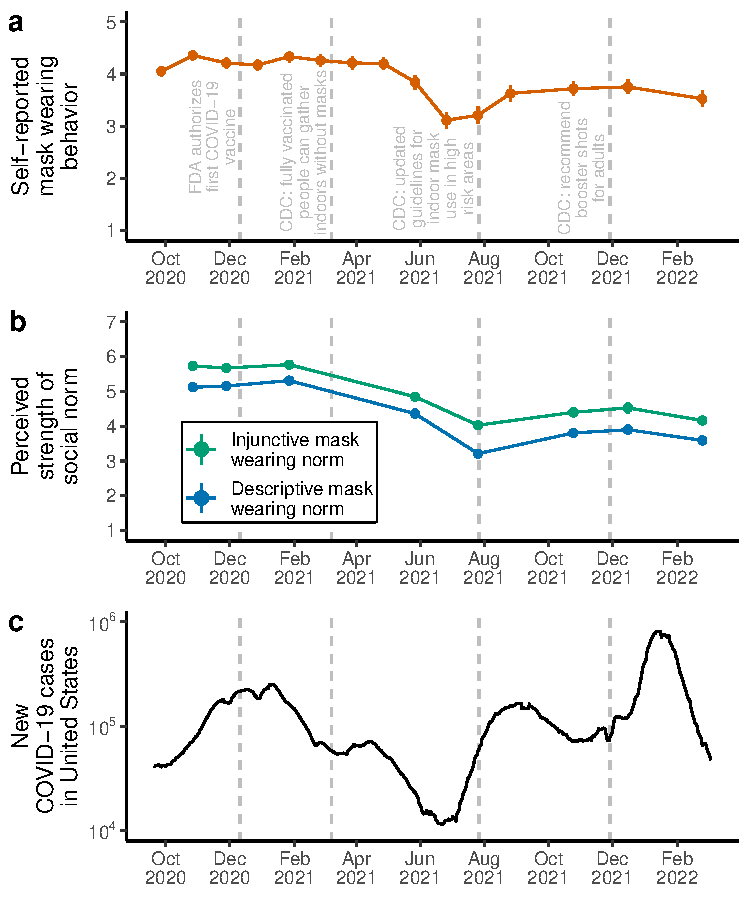
\includegraphics{manuscript_files/figure-latex/plotTimeline-1.pdf}
\caption{\label{fig:plotTimeline}\emph{Timeline of self-reported mask wearing and perceived social norms in the United States during the COVID-19 pandemic.} (a) Points and line ranges indicate means ± two standard errors for the self-reported mask wearing item. This item was measured across all eighteen time points on a 5-point Likert scale, with higher values indicating increased frequency of personal mask wearing during in-person interactions. (b) Points and line ranges indicate means ± two standard errors for perceived injunctive mask wearing norms (green) and perceived descriptive mask wearing norms (blue). These items were measured across eleven time points on a 7-point Likert scale, with higher values indicating stronger perceived social norms. (c) Smoothed data for daily new COVID-19 cases in the United States, displayed on the log scale (data retrieved from Our World in Data; \url{https://ourworldindata.org/}). Across all panels, gray dashed lines represent significant pandemic-related events in the United States, such as vaccine approval from the Food and Drug Administration (FDA) and public health recommendations from the Centers for Disease Control and Prevention (CDC).}
\end{figure}

Two main observations can be made about the emergence and stability of social norms from these visualizations. First, social norms and behavior were tightly coupled over time. Although social norms are measured on fewer occasions than mask wearing, we can see that as mask wearing decreased in the summer of 2021, so too did perceived descriptive and injunctive mask wearing norms. Subsequently, the steep rise in COVID-19 case numbers in the fall of 2021 saw concomitant increases in both mask wearing and perceived social norms, before declining again in 2022. In line with these patterns, multilevel regression models revealed positive correlations between mask wearing and perceived descriptive mask wearing norms (\emph{b} = 0.29, 95\% confidence interval {[}0.23 0.35{]}, \emph{p} \textless{} .001) and between mask wearing and perceived injunctive mask wearing norms (\emph{b} = 0.26, 95\% CI {[}0.22 0.30{]}, \emph{p} \textless{} .001) across individuals and time points (Supplementary Figure \ref{fig:plotCorBehNorm}; Supplementary Table \ref{tab:modelSummaryTable1}).

Second, fluctuations in mask wearing and perceived social norms are in line with recommendations broadcasted by the CDC, an important institution governing public health in the United States. We do not have data for the very start of the pandemic in early 2020, but the high levels of mask wearing and strong perceived social norms at the start of our observation window likely emerged after the initial mask wearing recommendation from the CDC in April 2020. Perceived social norms and mask wearing subsequently declined after the CDC rescinded their mask wearing recommendation following widespread vaccine availability in March 2021, and then increased again after the CDC updated their guidelines for indoor mask use in high-risk areas in August 2021. Finally, perceived social norms and mask wearing declined again after the CDC eased mask wearing guidelines in March 2022. These trends were confirmed by a series of multilevel regression models with change points aligning with changes in CDC mask wearing recommendations (Supplementary Figure \ref{fig:plotCDCSens}; Supplementary Table \ref{tab:changePointsTable}).

Sample averages can provide informative trends, but they do not allow us to estimate within-person changes in mask wearing and perceived social norms over time. To determine whether within-person changes in social norms temporally preceded within-person changes in mask wearing, we fitted a ten-wave unconstrained random-intercept cross-lagged panel model to the longitudinal data. This structural equation model separately estimated stable trait-like between-person individual differences and within-person fluctuations from those trait levels for our main variables (self-reported mask wearing, perceived descriptive mask wearing norms, and perceived injunctive mask wearing norms) and time-variant control variables (factual beliefs and personal normative beliefs). In line with our proposed causal model (Supplementary Figure \ref{fig:plotDAG}), we also included political orientation as an exogenous time-invariant control. According to established fit statistics, this model fitted the data well (root mean square error of approximation = 0.030, 95\% CI {[}0.028 0.033{]}; standardized root mean squared residual = 0.087; comparative fit index = 0.957). Since we are primarily interested in the causal effects of social norms on behavior, in what follows we focus on the results for mask wearing, perceived descriptive norms, and perceived injunctive norms (but see Supplementary Table \ref{tab:lavaanTable} for full list of estimated autoregressive and cross-lagged effects).

Regarding between-person individual differences, the covariances between the random intercepts in the model revealed positive correlations between stable trait levels of mask wearing and perceived social norms. On average across the whole study, participants who more frequently wore masks during in-person interactions also perceived stronger descriptive mask wearing norms (\emph{r} = 0.19, 95\% CI {[}0.04 0.33{]}, \emph{p} = .019) and stronger injunctive mask wearing norms (\emph{r} = 0.27, 95\% CI {[}0.14 0.40{]}, \emph{p} \textless{} .001). Stable trait perceptions of descriptive and injunctive mask wearing norms were also highly positively correlated (\emph{r} = 0.71, 95\% CI {[}0.65 0.78{]}, \emph{p} \textless{} .001).

Regarding within-person dynamics over time, Figure \ref{fig:plotRICLPM} displays autoregressive and cross-lagged effects for perceived descriptive norms, perceived injunctive norms, and mask wearing across the study duration, controlling for non-social beliefs and political orientation. In random intercept cross-lagged panel models, autoregressive effects represent ``persistence'' or ``inertia'' in within-person fluctuations from stable trait levels. In other words, a positive autoregressive effect indicates that being higher than average on one measure predicts being higher than average on that same measure in the following time point (this is not to be confused with the ``stable trait level'' over time, which is captured by the random intercepts in our model). For example, an autoregressive effect from mask wearing in February 2021 to future mask wearing in June 2021 would suggest that wearing masks more than average in February predicts wearing masks more than average in June. By contrast, and most relevant for the current study, cross-lagged effects represent the effect of a within-person fluctuation in one measure on future within-person fluctuations in other measures. In other words, a positive cross-lagged effect indicates that being higher than average on one measure predicts being higher than average on \emph{another} measure in the following time point. For example, a cross-lagged effect from descriptive norms in February 2021 to future mask wearing in June 2021 would suggest that perceiving descriptive norms as stronger than average in February predicts wearing masks more than average in June. Cross-lagged effects are thus used to infer within-person causal influences over time.



\begin{figure}
\centering
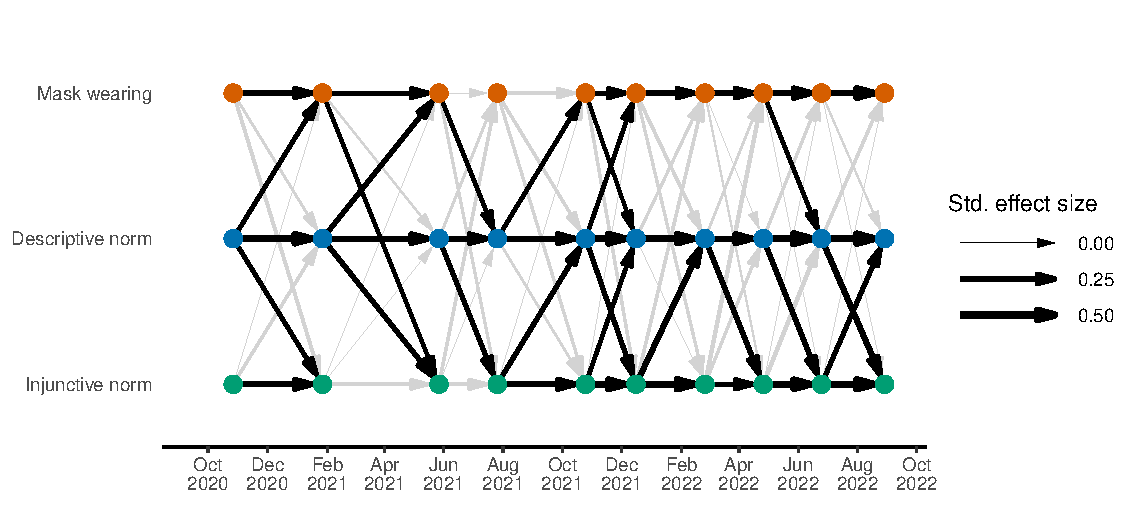
\includegraphics{manuscript_files/figure-latex/plotRICLPM-1.pdf}
\caption{\label{fig:plotRICLPM}\emph{Results of ten-wave unconstrained random-intercept cross-lagged panel model.} Circles represent data collection time points. Arrows represent within-person autoregressive effects (on one horizontal level) and cross-lagged effects (across levels) for mask wearing and perceived descriptive and injunctive norms, partitioning out stable between-person individual differences and controlling for factual beliefs, personal normative beliefs, and political orientation. Arrow thickness is scaled according to standardized effect size. Bolded arrows indicate significantly positive parameters, \emph{p} \textless{} 0.05. Gray arrows indicate non-significant parameters. There are no significant direct paths from injunctive norms to future mask wearing, showing that people's beliefs about what they should be doing did not have any direct influences on future mask wearing. On the other hand, there are significant paths from descriptive norms to future mask wearing, meaning that people's beliefs about what others are doing influenced their future mask wearing.}
\end{figure}

In late 2020 and throughout 2021, we see several cross-lagged effects from perceived descriptive norms to future mask wearing. On four occasions, within-person increases in perceived descriptive norms predicted future within-person increases in mask wearing. According to recent effect size guidelines for cross-lagged panel models (Orth et al., 2022), the standardized beta coefficients for these cross-lagged effects were large (first wave, \(\beta\) = 0.17, 95\% CI {[}0.06 0.28{]}, \emph{p} = .002; second wave, \(\beta\) = 0.21, 95\% CI {[}0.08 0.34{]}, \emph{p} = .001; fourth wave, \(\beta\) = 0.15, 95\% CI {[}0.01 0.30{]}, \emph{p} = .041; fifth wave, \(\beta\) = 0.16, 95\% CI {[}0.02 0.29{]}, \emph{p} = .023). In 2022, these cross-lagged effects from descriptive norms to mask wearing diminished. We also find some evidence for a reciprocal effect, whereby within-person increases in mask wearing predicted future within-person increases in perceived descriptive norms. Moreover, several cross-lagged effects emerged between perceived descriptive and injunctive norms, demonstrating reciprocal within-person causal effects between these variables.

However, the model also reveals that, after controlling for perceived descriptive norms, non-social beliefs, and political orientation, within-person changes in perceived injunctive norms did \emph{not} predict future within-person changes in mask wearing across our study duration. All cross-lagged effects from perceived injunctive norms to mask wearing are non-significant. Any causal effect that perceived injunctive norms might have had on future mask wearing appears to be fully mediated by perceived descriptive norms. This means that believing that others think that mask wearing is the right thing to do influences one's perception of what others are actually doing, which then influences future behavior. For example, between August 2021 and December 2021, perceived injunctive norms predicted future perceived descriptive norms, which themselves predicted future mask wearing. But aside from these indirect effects, perceived injunctive norms did not have a direct causal effect on mask wearing over time within individuals.

\hypertarget{discussion}{%
\section{Discussion}\label{discussion}}

Using longitudinal data from the United States across two years of the COVID-19 pandemic, we aimed to understand how descriptive and injunctive mask wearing norms emerge and influence behavior in response to a naturally unfolding social dilemma. The trends of norm perceptions and self-reported mask wearing over time suggest that norms and behavior were tightly coupled and both changed dynamically in response to recommendations from public health authorities. Moreover, the results of our cross-lagged panel model indicate that descriptive norms caused future increases in mask wearing in the first year and a half of the pandemic. By contrast, injunctive norms were not directly causally related to future mask wearing over the entire two years of data collection.

Our finding that social norms and mask wearing are tightly coupled over time provides real-world support for experimental evidence that social norms and cooperative behavior develop synergistically within groups via processes of social interaction (Titlestad et al., 2019). The fact that these changes closely tracked the release of guidelines by the CDC supports the idea that institutions are part of the process by which culture and one's own behaviors are mutually constructed (Markus \& Kitayama, 2010). Indeed, empirical work in cultural evolution suggests that formal institutions are critical for the emergence and rapid adoption of novel social norms (Amato et al., 2018). While new norms can and do emerge spontaneously in populations, the process is slow compared to institution-driven norm change, which, as our trends have shown, can unfold over measurement intervals as short as four to six weeks.

We found that descriptive norms, not injunctive norms, predicted future within-person increases in mask wearing, independent of the effects of non-social beliefs and political orientation. This finding is in line with previous evidence showing that perceptions of descriptive norms were positively related to other protective COVID-19 behaviors (Bokemper et al., 2021; Rudert \& Janke, 2021). There are several explanations for why descriptive norms have had these positive effects on protective COVID-19 behaviors like mask wearing. First, people may have followed descriptive norms to quickly coordinate their behavior with others during the pandemic. Descriptive norms are particularly useful for coordinating behavior during fast changing, threatening situations with a high degree of uncertainty, such as the COVID-19 pandemic (Gelfand \& Harrington, 2015). Second, people might have engaged in conditional cooperation, adapting their cooperation levels to the degree of cooperation in the population (Chaudhuri, 2011). Descriptive mask wearing norms provide evidence that others are cooperating, increasing the likelihood that individuals will themselves contribute to the public good by wearing masks. Third, the increased frequency of mask wearing in the population might have created a bandwagon effect (Schmitt-Beck, 2015), encouraging conformist copying. Under this view, people wear masks not to coordinate or cooperate, but simply to fit in with the crowd. Future research will be required to determine the motivations underlying adherence to descriptive norms during uncertain times.

We found that perceived injunctive norms did not directly predict future within-person increases in mask wearing, suggesting that injunctive norms and mask wearing are not directly causally related. One possible explanation for this result is that, due to the increased opportunities to observe mask wearing in public, descriptive norms of mask wearing were more salient than injunctive norms during the pandemic. According to focus theory (Cialdini et al., 1991), this difference in salience would produce behavior in line with descriptive norms and potentially suppress the effects of injunctive norms. By contrast, for more private behaviors like remaining indoors, it would have been less possible to observe other people's behaviors, increasing the relative salience of injunctive norms. To test this idea, future research should expand our longitudinal approach to protective behaviors beyond mask wearing, including both public behaviors (e.g., physical distancing) and private behaviors (e.g., hand washing and home isolation).

We are limited in generalizing these findings due to the constraints of our sample and the variables considered. While our sample began as representative of the United States, there was significant attrition over the course of the study (Supplementary Figure \ref{fig:plotAttrition}). This attrition did not leave us with enough data to test the robustness of our results within different identity groups, such as different genders, ethnicities, or political ideologies. Our results also might not generalize to all social norms, behaviors, and social dilemmas. Norms governing sustainability in response to climate change, for example, might take longer to emerge, since the threat of climate change is more remote than the COVID-19 pandemic. For more distant social dilemmas that do not cause immediate day-to-day uncertainty, descriptive social norms may not necessarily drive cooperative behavior.

For the case of mask wearing in the United States during the COVID-19 pandemic, we have shown that social norms developed rapidly in the population and tracked ongoing changes in both recommendations from authorities and current levels of cooperative behavior. Moreover, we found that descriptive norms, rather than injunctive norms, were the main driver for future mask wearing. Our work thus underscores the importance of consistent, visible community adherence for encouraging protective behaviors in response to global pandemics like COVID-19.

\newpage

\hypertarget{acknowledgements}{%
\section{Acknowledgements}\label{acknowledgements}}

{[}REDACTED{]}

\hypertarget{author-contributions}{%
\section{Author Contributions}\label{author-contributions}}

{[}REDACTED{]}

\hypertarget{conflicts-of-interest}{%
\section{Conflicts of Interest}\label{conflicts-of-interest}}

There are no conflicts of interest to declare.

\hypertarget{open-practices-statement}{%
\section{Open Practices Statement}\label{open-practices-statement}}

All data and code to reproduce the statistical analyses in this manuscript are publicly available on GitHub: \url{https://github.com/ScottClaessens/covidMaskWearing} This study was not preregistered.

\newpage

\hypertarget{references}{%
\section{References}\label{references}}

\begingroup

\hypertarget{refs}{}
\begin{CSLReferences}{1}{0}
\leavevmode\vadjust pre{\hypertarget{ref-Amato2018}{}}%
Amato, R., Lacasa, L., Díaz-Guilera, A., \& Baronchelli, A. (2018). The dynamics of norm change in the cultural evolution of language. \emph{Proceedings of the National Academy of Sciences}, \emph{115}(33), 8260--8265. \url{https://doi.org/10.1073/pnas.1721059115}

\leavevmode\vadjust pre{\hypertarget{ref-Aust2022}{}}%
Aust, F., \& Barth, M. (2022). \emph{{papaja}: {Prepare} reproducible {APA} journal articles with {R Markdown}}. \url{https://github.com/crsh/papaja}

\leavevmode\vadjust pre{\hypertarget{ref-Bates2015}{}}%
Bates, D., Mächler, M., Bolker, B., \& Walker, S. (2015). Fitting linear mixed-effects models using lme4. \emph{Journal of Statistical Software}, \emph{67}(1), 1--48. \url{https://doi.org/10.18637/jss.v067.i01}

\leavevmode\vadjust pre{\hypertarget{ref-BaxterKing2022}{}}%
Baxter-King, R., Brown, J. R., Enos, R. D., Naeim, A., \& Vavreck, L. (2022). How local partisan context conditions prosocial behaviors: Mask wearing during {COVID-19}. \emph{Proceedings of the National Academy of Sciences}, \emph{119}(21), e2116311119. \url{https://doi.org/10.1073/pnas.2116311119}

\leavevmode\vadjust pre{\hypertarget{ref-Bicchieri2014}{}}%
Bicchieri, C., Lindemans, J. W., \& Jiang, T. (2014). A structured approach to a diagnostic of collective practices. \emph{Frontiers in Psychology}, \emph{5}, 1418. \url{https://doi.org/10.3389/fpsyg.2014.01418}

\leavevmode\vadjust pre{\hypertarget{ref-Bicchieri2009}{}}%
Bicchieri, C., \& Xiao, E. (2009). Do the right thing: But only if others do so. \emph{Journal of Behavioral Decision Making}, \emph{22}(2), 191--208. \url{https://doi.org/10.1002/bdm.621}

\leavevmode\vadjust pre{\hypertarget{ref-Bokemper2021}{}}%
Bokemper, S. E., Cucciniello, M., Rotesi, T., Pin, P., Malik, A. A., Willebrand, K., Paintsil, E. E., Omer, S. B., Huber, G. A., \& Melegaro, A. (2021). Experimental evidence that changing beliefs about mask efficacy and social norms increase mask wearing for {COVID-19} risk reduction: Results from the {United States} and {Italy}. \emph{PLOS ONE}, \emph{16}(10), e0258282. \url{https://doi.org/10.1371/journal.pone.0258282}

\leavevmode\vadjust pre{\hypertarget{ref-CDC2020}{}}%
Centers for Disease Control and Prevention. (2020). \emph{{CDC calls on Americans to wear masks to prevent COVID-19 spread}}. \url{https://www.cdc.gov/media/releases/2020/p0714-americans-to-wear-masks.html}

\leavevmode\vadjust pre{\hypertarget{ref-CDC2022}{}}%
Centers for Disease Control and Prevention. (2022). \emph{{CDC Museum COVID-19 Timeline}}. \url{https://www.cdc.gov/museum/timeline/covid19.html}

\leavevmode\vadjust pre{\hypertarget{ref-Chaudhuri2011}{}}%
Chaudhuri, A. (2011). Sustaining cooperation in laboratory public goods experiments: A selective survey of the literature. \emph{Experimental Economics}, \emph{14}(1), 47--83. \url{https://doi.org/10.1007/s10683-010-9257-1}

\leavevmode\vadjust pre{\hypertarget{ref-Cialdini2021}{}}%
Cialdini, R. B., \& Jacobson, R. P. (2021). Influences of social norms on climate change-related behaviors. \emph{Current Opinion in Behavioral Sciences}, \emph{42}, 1--8. \url{https://doi.org/10.1016/j.cobeha.2021.01.005}

\leavevmode\vadjust pre{\hypertarget{ref-Cialdini1991}{}}%
Cialdini, R. B., Kallgren, C. A., \& Reno, R. R. (1991). \emph{A focus theory of normative conduct: A theoretical refinement and reevaluation of the role of norms in human behavior} (M. P. Zanna, Ed.; Vol. 24, pp. 201--234). Academic Press. \url{https://doi.org/10.1016/S0065-2601(08)60330-5}

\leavevmode\vadjust pre{\hypertarget{ref-Deutsch1955}{}}%
Deutsch, M., \& Gerard, H. B. (1955). A study of normative and informational social influences upon individual judgment. \emph{The Journal of Abnormal and Social Psychology}, \emph{51}(3), 629--636. \url{https://doi.org/10.1037/h0046408}

\leavevmode\vadjust pre{\hypertarget{ref-Fehr2018a}{}}%
Fehr, E., \& Schurtenberger, I. (2018). Normative foundations of human cooperation. \emph{Nature Human Behaviour}, \emph{2}(7), 458--468. \url{https://doi.org/10.1038/s41562-018-0385-5}

\leavevmode\vadjust pre{\hypertarget{ref-Gelfand2015}{}}%
Gelfand, M. J., \& Harrington, J. R. (2015). The motivational force of descriptive norms: For whom and when are descriptive norms most predictive of behavior? \emph{Journal of Cross-Cultural Psychology}, \emph{46}(10), 1273--1278. \url{https://doi.org/10.1177/0022022115600796}

\leavevmode\vadjust pre{\hypertarget{ref-Goldstein2008}{}}%
Goldstein, N. J., Cialdini, R. B., \& Griskevicius, V. (2008). A room with a viewpoint: Using social norms to motivate environmental conservation in hotels. \emph{Journal of Consumer Research}, \emph{35}(3), 472--482. \url{https://doi.org/10.1086/586910}

\leavevmode\vadjust pre{\hypertarget{ref-Granger1969}{}}%
Granger, C. W. J. (1969). Investigating causal relations by econometric models and cross-spectral methods. \emph{Econometrica}, \emph{37}(3), 424--438. \url{https://doi.org/10.2307/1912791}

\leavevmode\vadjust pre{\hypertarget{ref-Hamaker2015}{}}%
Hamaker, E. L., Kuiper, R. M., \& Grasman, R. P. P. P. (2015). A critique of the cross-lagged panel model. \emph{Psychological Methods}, \emph{20}(1), 102--116. \url{https://doi.org/10.1037/a0038889}

\leavevmode\vadjust pre{\hypertarget{ref-Heiman2023}{}}%
Heiman, S. L., Claessens, S., Ayers, J. D., Beltrán, D. G., Van Horn, A., Hirt, E. R., Aktipis, A., \& Todd, P. M. (2023). \emph{Descriptive, not injunctive, social norms caused increases in mask wearing during the COVID-19 pandemic}. GitHub repository. \url{https://github.com/ScottClaessens/covidMaskWearing}

\leavevmode\vadjust pre{\hypertarget{ref-Henrich2015}{}}%
Henrich, J. (2015). \emph{The secret of our success: How culture is driving human evolution, domesticating our species, and making us smarter}. Princeton University Press. \url{https://doi.org/10.2307/j.ctvc77f0d}

\leavevmode\vadjust pre{\hypertarget{ref-Landau2021}{}}%
Landau, W. M. (2021). The targets {R} package: A dynamic {M}ake-like function-oriented pipeline toolkit for reproducibility and high-performance computing. \emph{Journal of Open Source Software}, \emph{6}(57), 2959. \url{https://doi.org/10.21105/joss.02959}

\leavevmode\vadjust pre{\hypertarget{ref-Larkin2018}{}}%
Larkin, C., Sanders, M., Andresen, I., \& Algate, F. (2018). \emph{Testing local descriptive norms and salience of enforcement action: A field experiment to increase tax collection} (SSRN Scholarly Paper No. 3167575). \url{https://doi.org/10.2139/ssrn.3167575}

\leavevmode\vadjust pre{\hypertarget{ref-Legros2020}{}}%
Legros, S., \& Cislaghi, B. (2020). Mapping the social-norms literature: An overview of reviews. \emph{Perspectives on Psychological Science}, \emph{15}(1), 62--80. \url{https://doi.org/10.1177/1745691619866455}

\leavevmode\vadjust pre{\hypertarget{ref-Macy2021}{}}%
Macy, J. T., Owens, C., Mullis, K., \& Middlestadt, S. E. (2021). The role of self-efficacy and injunctive norms in helping older adults decide to stay home during the {COVID-19} pandemic. \emph{Frontiers in Public Health}, \emph{9}, 660813. \url{https://doi.org/10.3389/fpubh.2021.660813}

\leavevmode\vadjust pre{\hypertarget{ref-Markus2010}{}}%
Markus, H. R., \& Kitayama, S. (2010). Cultures and selves: A cycle of mutual constitution. \emph{Perspectives on Psychological Science}, \emph{5}(4), 420--430. \url{https://doi.org/10.1177/1745691610375557}

\leavevmode\vadjust pre{\hypertarget{ref-Nigbur2010}{}}%
Nigbur, D., Lyons, E., \& Uzzell, D. (2010). Attitudes, norms, identity and environmental behaviour: Using an expanded theory of planned behaviour to predict participation in a kerbside recycling programme. \emph{British Journal of Social Psychology}, \emph{49}(2), 259--284. \url{https://doi.org/10.1348/014466609X449395}

\leavevmode\vadjust pre{\hypertarget{ref-Orth2022}{}}%
Orth, U., Meier, L. L., Bühler, J. L., Dapp, L. C., Krauss, S., Messerli, D., \& Robins, R. W. (2022). Effect size guidelines for cross-lagged effects. \emph{Psychological Methods}. \url{https://doi.org/10.1037/met0000499}

\leavevmode\vadjust pre{\hypertarget{ref-RCoreTeam}{}}%
R Core Team. (2022). \emph{R: A language and environment for statistical computing}. R Foundation for Statistical Computing. \url{https://www.R-project.org/}

\leavevmode\vadjust pre{\hypertarget{ref-Roos2015}{}}%
Roos, P., Gelfand, M., Nau, D., \& Lun, J. (2015). Societal threat and cultural variation in the strength of social norms: An evolutionary basis. \emph{Organizational Behavior and Human Decision Processes}, \emph{129}, 14--23. \url{https://doi.org/10.1016/j.obhdp.2015.01.003}

\leavevmode\vadjust pre{\hypertarget{ref-Rosseel2012}{}}%
Rosseel, Y. (2012). {lavaan}: An {R} package for structural equation modeling. \emph{Journal of Statistical Software}, \emph{48}(2), 1--36. \url{https://doi.org/10.18637/jss.v048.i02}

\leavevmode\vadjust pre{\hypertarget{ref-Rudert2021}{}}%
Rudert, S. C., \& Janke, S. (2021). Following the crowd in times of crisis: Descriptive norms predict physical distancing, stockpiling, and prosocial behavior during the {COVID-19} pandemic. \emph{Group Processes \& Intergroup Relations}, \emph{25}, 1819--1835. \url{https://doi.org/10.1177/13684302211023562}

\leavevmode\vadjust pre{\hypertarget{ref-SchmittBeck2015}{}}%
Schmitt-Beck, R. (2015). Bandwagon effect. In \emph{The international encyclopedia of political communication} (pp. 1--5). John Wiley \& Sons, Ltd. \url{https://doi.org/10.1002/9781118541555.wbiepc015}

\leavevmode\vadjust pre{\hypertarget{ref-Schultz2007}{}}%
Schultz, P. W., Nolan, J. M., Cialdini, R. B., Goldstein, N. J., \& Griskevicius, V. (2007). The constructive, destructive, and reconstructive power of social norms. \emph{Psychological Science}, \emph{18}(5), 429--434. \url{https://doi.org/10.1111/j.1467-9280.2007.01917.x}

\leavevmode\vadjust pre{\hypertarget{ref-Smith2015}{}}%
Smith, L. G. E., Thomas, E. F., \& McGarty, C. (2015). "We must be the change we want to see in the world": Integrating norms and identities through social interaction. \emph{Political Psychology}, \emph{36}(5), 543--557. \url{https://doi.org/10.1111/pops.12180}

\leavevmode\vadjust pre{\hypertarget{ref-Titlestad2019}{}}%
Titlestad, K., Snijders, T. A. B., Durrheim, K., Quayle, M., \& Postmes, T. (2019). The dynamic emergence of cooperative norms in a social dilemma. \emph{Journal of Experimental Social Psychology}, \emph{84}, 103799. \url{https://doi.org/10.1016/j.jesp.2019.03.010}

\leavevmode\vadjust pre{\hypertarget{ref-VanKleef2019}{}}%
van Kleef, G. A., Gelfand, M. J., \& Jetten, J. (2019). The dynamic nature of social norms: New perspectives on norm development, impact, violation, and enforcement. \emph{Journal of Experimental Social Psychology}, \emph{84}, 103814. \url{https://doi.org/10.1016/j.jesp.2019.05.002}

\leavevmode\vadjust pre{\hypertarget{ref-Wickham2016}{}}%
Wickham, H. (2016). \emph{{ggplot2}: Elegant graphics for data analysis}. Springer-Verlag New York. \url{https://ggplot2.tidyverse.org}

\leavevmode\vadjust pre{\hypertarget{ref-Wilke2020}{}}%
Wilke, C. O. (2020). \emph{{cowplot}: Streamlined plot theme and plot annotations for 'ggplot2'}. \url{https://CRAN.R-project.org/package=cowplot}

\end{CSLReferences}

\endgroup

\newpage

\hypertarget{appendix-appendix}{%
\appendix}


\renewcommand{\appendixname}{\textbf{Supplementary Material}}
\renewcommand{\thefigure}{S\arabic{figure}} \setcounter{figure}{0}
\renewcommand{\thetable}{S\arabic{table}} \setcounter{table}{0}
\renewcommand{\theequation}{S\arabic{table}} \setcounter{equation}{0}

\hypertarget{section}{%
\section{}\label{section}}

\hypertarget{supplementary-results}{%
\subsection{Supplementary Results}\label{supplementary-results}}

\hypertarget{construct-validity-for-measures-of-perceived-descriptive-and-injunctive-norms}{%
\subsubsection{Construct validity for measures of perceived descriptive and injunctive norms}\label{construct-validity-for-measures-of-perceived-descriptive-and-injunctive-norms}}

To evaluate the construct validity of our measures of perceived descriptive and injunctive norms, at Time 7 we asked participants to rate the extent to which each perceived norm item provided descriptive and injunctive information. For each item, participants were asked whether the item provided information about what people \emph{are} doing, and whether the item provided information about what people \emph{should} be doing. Participants responded on a 7-point Likert scale, from (1) Not At All to (7) Very Strongly. For a full list of questions, see Supplementary Table \ref{tab:itemTable}.

Results showed that participants did differentiate the perceived norm items as expected. Participants rated the perceived descriptive norm items as providing more descriptive information than the perceived injunctive norm items, \emph{t}(442) = -7.28, \emph{p} \textless{} .001 (mean descriptive items = 4.75; mean injunctive items = 4.25). By contrast, participants rated the perceived injunctive norm items as providing more injunctive information than the perceived descriptive norm items, \emph{t}(444) = 7.15, \emph{p} \textless{} .001 (mean descriptive items = 5.11; mean injunctive items = 5.54).

\newpage

\hypertarget{supplementary-figures}{%
\subsection{Supplementary Figures}\label{supplementary-figures}}



\begin{figure}
\centering
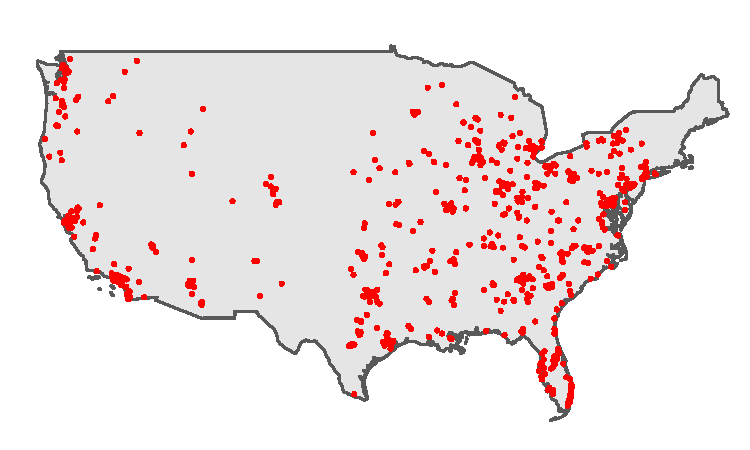
\includegraphics{manuscript_files/figure-latex/plotUSMap-1.pdf}
\caption{\label{fig:plotUSMap}\emph{Map of the United States with participant zip code locations.}}
\end{figure}

\newpage



\begin{figure}
\centering
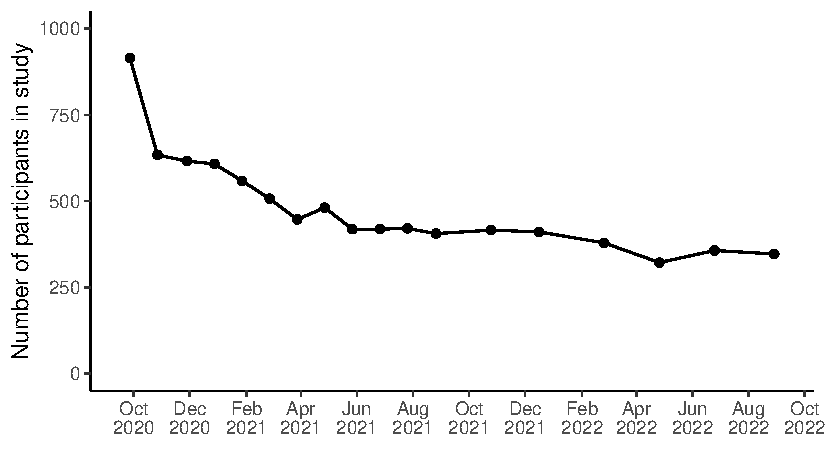
\includegraphics{manuscript_files/figure-latex/plotAttrition-1.pdf}
\caption{\label{fig:plotAttrition}\emph{Attrition across the course of the study.}}
\end{figure}

\newpage



\begin{figure}
\centering
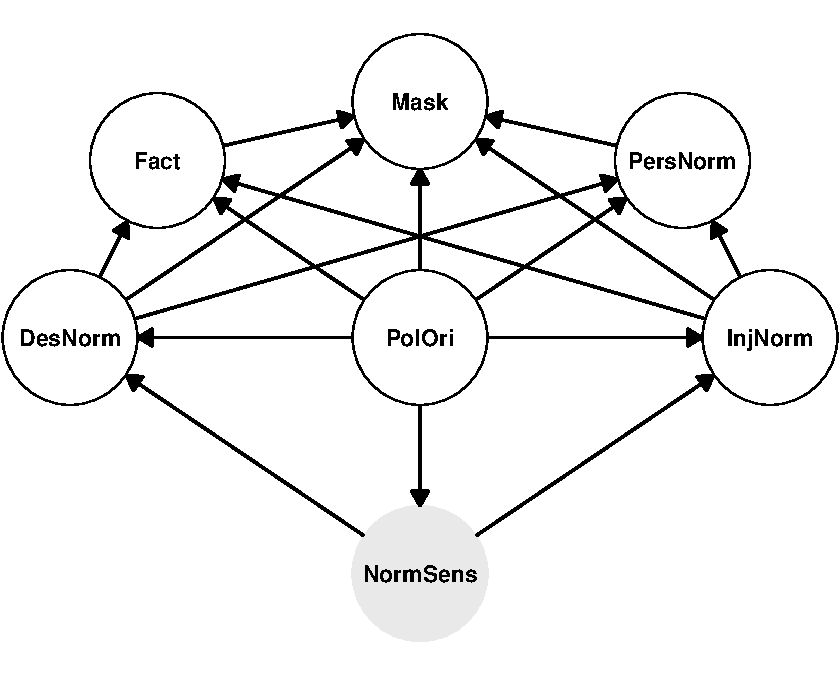
\includegraphics{manuscript_files/figure-latex/plotDAG-1.pdf}
\caption{\label{fig:plotDAG}\emph{Directed acyclic graph reflecting causal assumptions.} In this model, a general unobserved sensitivity to social norms (NormSens) causes perceptions of descriptive social norms (DesNorm) and perceptions of injunctive social norms (InjNorm), and perceptions of descriptive and injunctive norms directly cause mask wearing (Mask). Perceptions of descriptive and injunctive norms also indirectly cause mask wearing through non-social beliefs, specifically factual beliefs (Fact) and personal normative beliefs (PersNorm). Finally, political orientation (PolOri) is an exogenous variable that is a common cause of all other variables. Using the backdoor criterion (Pearl, 1995), this causal model implies that it is necessary to control for perceptions of injunctive norms, factual beliefs, personal normative beliefs, and political orientation to estimate the direct causal effect of perceived descriptive norms on mask wearing. Similarly, it is necessary to control for perceptions of descriptive norms, factual beliefs, personal normative beliefs, and political orientation to estimate the direct causal effect of perceived injunctive norms on mask wearing.}
\end{figure}

\newpage



\begin{figure}
\centering
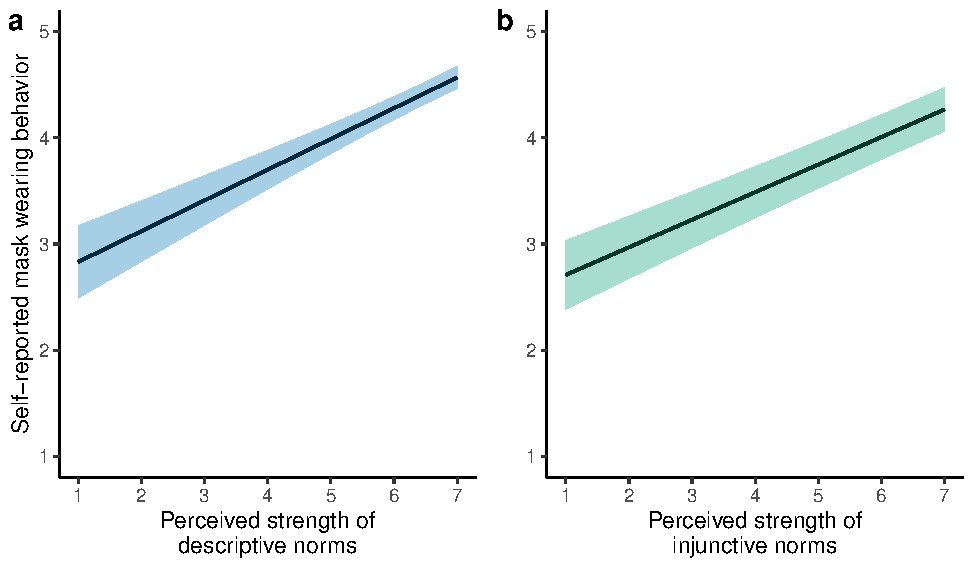
\includegraphics{manuscript_files/figure-latex/plotCorBehNorm-1.pdf}
\caption{\label{fig:plotCorBehNorm}\emph{Predictions from multilevel models with self-reported mask wearing as the outcome variable and (a) perceived strength of descriptive norms and (b) perceived strength of injunctive norms as independent predictor variables.} Models contain random intercepts for participants and time points. Lines are fixed effect regression lines from multilevel models, shaded areas are 95\% confidence intervals.}
\end{figure}

\newpage



\begin{figure}
\centering
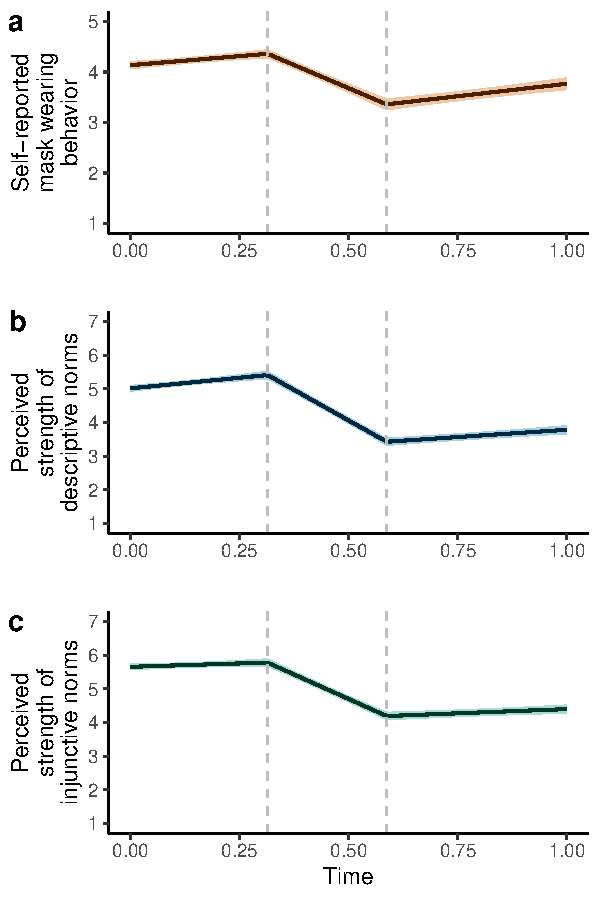
\includegraphics{manuscript_files/figure-latex/plotCDCSens-1.pdf}
\caption{\label{fig:plotCDCSens}\emph{Predictions from multilevel models with change points in line with changes in CDC mask wearing recommendations.} These models track temporal changes in (a) self-reported mask wearing, (b) perceived strength of descriptive norms, and (c) perceived strength of injunctive norms. Time is included as a continuous linear predictor, scaled between 0 and 1, with three forced change points (dashed lines). From the left, the first dashed line indicates when the CDC relaxed their mask wearing recommendations in March 2021, the second dashed line indicates when the CDC strengthened their mask wearing recommendations in July 2021, and the third dashed line indicates when the CDC updated their community levels and relaxed their mask wearing recommendations in March 2022. This results in the estimation of five fixed effect parameters: the initial intercept, the slope in the first window, the slope in the second window, the slope in the third window, and the slope is the fourth window. Bolded lines and shaded areas represent fixed effect regression lines from multilevel models and 95\% confidence intervals, respectively.}
\end{figure}

\newpage

\hypertarget{supplementary-tables}{%
\subsection{Supplementary Tables}\label{supplementary-tables}}



\begin{center}
\begin{ThreePartTable}

\begin{longtable}{m{2.5cm}m{2.5cm}m{9cm}}\noalign{\getlongtablewidth\global\LTcapwidth=\longtablewidth}
\caption{\label{tab:itemTable}List of norm interpretation questions asked at Time 7. \emph{These questions were preceded by the following text:} ``There may or may not be a difference between what people around you are doing and what they should be doing. You can learn about what people are doing and what they should be doing in different ways. For each of the following information sources, we want to know if you can learn from it what people are doing, what people should be doing, or both''. \emph{Participants answered all questions on a 7-point Likert scale, from (1) Not At All to (7) Very Strongly.}}\\
\toprule
Interpretation & \multicolumn{1}{c}{Perceived norm item} & \multicolumn{1}{c}{Question}\\
\midrule
\endfirsthead
\caption*{\normalfont{Table \ref{tab:itemTable} continued}}\\
\toprule
Interpretation & \multicolumn{1}{c}{Perceived norm item} & \multicolumn{1}{c}{Question}\\
\midrule
\endhead
Provides descriptive information & Descriptive & Does noticing the proportion of people in your area that wear a mask while doing recreational/social activities indoors (e.g., going to the gym, eating at a restaurant, attending a party) tell you what everyone is doing?\\
 &  & Does noticing the proportion of people in your area that wear a mask while doing routine activities indoors (e.g., running errands, shopping, going to work) tell you what everyone is doing?\\
 & Injunctive & Do mask-wearing rules encouraged in your area (e.g., by local or state government officials, businesses, etc.) tell you what everyone is doing?\\
 &  & Does how often you see people that you respect and trust wearing a mask (e.g., on tv, news, etc.) tell you what everyone is doing?\\
Provides injunctive information & Descriptive & Does noticing the proportion of people in your area that wear a mask while doing recreational/social activities indoors (e.g., going to the gym, eating at a restaurant, attending a party) tell you what everyone should be doing?\\
 &  & Does noticing the proportion of people in your area that wear a mask while doing routine activities indoors (e.g., running errands, shopping, going to work) tell you what everyone should be doing?\\
 & Injunctive & Do mask-wearing rules encouraged in your area (e.g., by local or state government officials, businesses, etc.) tell you what everyone should be doing?\\
 &  & Does how often you see people that you respect and trust wearing a mask (e.g., on tv, news, etc.) tell you what everyone should be doing?\\
\bottomrule
\end{longtable}

\end{ThreePartTable}
\end{center}

\newpage



 
  \providecommand{\huxb}[2]{\arrayrulecolor[RGB]{#1}\global\arrayrulewidth=#2pt}
  \providecommand{\huxvb}[2]{\color[RGB]{#1}\vrule width #2pt}
  \providecommand{\huxtpad}[1]{\rule{0pt}{#1}}
  \providecommand{\huxbpad}[1]{\rule[-#1]{0pt}{#1}}

\begin{table}[ht]
\begin{centerbox}
\begin{threeparttable}
\captionsetup{justification=centering,singlelinecheck=off}
\caption{Unstandardized fixed effect parameters from multilevel models: perceptions of social norm strength predicting self-reported mask wearing. \emph{Standard errors are included in brackets.}}
 \label{tab:modelSummaryTable1}
\setlength{\tabcolsep}{0pt}
\begin{tabular}{l l l}


\hhline{>{\huxb{0, 0, 0}{0.8}}->{\huxb{0, 0, 0}{0.8}}->{\huxb{0, 0, 0}{0.8}}-}
\arrayrulecolor{black}

\multicolumn{1}{!{\huxvb{0, 0, 0}{0}}c!{\huxvb{0, 0, 0}{0}}}{\huxtpad{6pt + 1em}\centering \hspace{6pt}  \hspace{6pt}\huxbpad{6pt}} &
\multicolumn{1}{c!{\huxvb{0, 0, 0}{0}}}{\huxtpad{6pt + 1em}\centering \hspace{6pt} Model 1 \hspace{6pt}\huxbpad{6pt}} &
\multicolumn{1}{c!{\huxvb{0, 0, 0}{0}}}{\huxtpad{6pt + 1em}\centering \hspace{6pt} Model 2 \hspace{6pt}\huxbpad{6pt}} \tabularnewline[-0.5pt]


\hhline{>{\huxb{255, 255, 255}{0.4}}->{\huxb{0, 0, 0}{0.4}}->{\huxb{0, 0, 0}{0.4}}-}
\arrayrulecolor{black}

\multicolumn{1}{!{\huxvb{0, 0, 0}{0}}l!{\huxvb{0, 0, 0}{0}}}{\huxtpad{6pt + 1em}\raggedright \hspace{6pt} Intercept \hspace{6pt}\huxbpad{6pt}} &
\multicolumn{1}{r!{\huxvb{0, 0, 0}{0}}}{\huxtpad{6pt + 1em}\raggedleft \hspace{6pt} 2.54\hphantom{0} \hspace{6pt}\huxbpad{6pt}} &
\multicolumn{1}{r!{\huxvb{0, 0, 0}{0}}}{\huxtpad{6pt + 1em}\raggedleft \hspace{6pt} 2.45\hphantom{0} \hspace{6pt}\huxbpad{6pt}} \tabularnewline[-0.5pt]


\hhline{}
\arrayrulecolor{black}

\multicolumn{1}{!{\huxvb{0, 0, 0}{0}}l!{\huxvb{0, 0, 0}{0}}}{\huxtpad{6pt + 1em}\raggedright \hspace{6pt}  \hspace{6pt}\huxbpad{6pt}} &
\multicolumn{1}{r!{\huxvb{0, 0, 0}{0}}}{\huxtpad{6pt + 1em}\raggedleft \hspace{6pt} (0.20) \hspace{6pt}\huxbpad{6pt}} &
\multicolumn{1}{r!{\huxvb{0, 0, 0}{0}}}{\huxtpad{6pt + 1em}\raggedleft \hspace{6pt} (0.18) \hspace{6pt}\huxbpad{6pt}} \tabularnewline[-0.5pt]


\hhline{}
\arrayrulecolor{black}

\multicolumn{1}{!{\huxvb{0, 0, 0}{0}}l!{\huxvb{0, 0, 0}{0}}}{\huxtpad{6pt + 1em}\raggedright \hspace{6pt} Descriptive norms \hspace{6pt}\huxbpad{6pt}} &
\multicolumn{1}{r!{\huxvb{0, 0, 0}{0}}}{\huxtpad{6pt + 1em}\raggedleft \hspace{6pt} 0.29\hphantom{0} \hspace{6pt}\huxbpad{6pt}} &
\multicolumn{1}{r!{\huxvb{0, 0, 0}{0}}}{\huxtpad{6pt + 1em}\raggedleft \hspace{6pt} \hphantom{0}\hphantom{0}\hphantom{0}\hphantom{0} \hspace{6pt}\huxbpad{6pt}} \tabularnewline[-0.5pt]


\hhline{}
\arrayrulecolor{black}

\multicolumn{1}{!{\huxvb{0, 0, 0}{0}}l!{\huxvb{0, 0, 0}{0}}}{\huxtpad{6pt + 1em}\raggedright \hspace{6pt}  \hspace{6pt}\huxbpad{6pt}} &
\multicolumn{1}{r!{\huxvb{0, 0, 0}{0}}}{\huxtpad{6pt + 1em}\raggedleft \hspace{6pt} (0.03) \hspace{6pt}\huxbpad{6pt}} &
\multicolumn{1}{r!{\huxvb{0, 0, 0}{0}}}{\huxtpad{6pt + 1em}\raggedleft \hspace{6pt} \hphantom{0}\hphantom{0}\hphantom{0}\hphantom{0} \hspace{6pt}\huxbpad{6pt}} \tabularnewline[-0.5pt]


\hhline{}
\arrayrulecolor{black}

\multicolumn{1}{!{\huxvb{0, 0, 0}{0}}l!{\huxvb{0, 0, 0}{0}}}{\huxtpad{6pt + 1em}\raggedright \hspace{6pt} Injunctive norms \hspace{6pt}\huxbpad{6pt}} &
\multicolumn{1}{r!{\huxvb{0, 0, 0}{0}}}{\huxtpad{6pt + 1em}\raggedleft \hspace{6pt} \hphantom{0}\hphantom{0}\hphantom{0}\hphantom{0} \hspace{6pt}\huxbpad{6pt}} &
\multicolumn{1}{r!{\huxvb{0, 0, 0}{0}}}{\huxtpad{6pt + 1em}\raggedleft \hspace{6pt} 0.26\hphantom{0} \hspace{6pt}\huxbpad{6pt}} \tabularnewline[-0.5pt]


\hhline{}
\arrayrulecolor{black}

\multicolumn{1}{!{\huxvb{0, 0, 0}{0}}l!{\huxvb{0, 0, 0}{0}}}{\huxtpad{6pt + 1em}\raggedright \hspace{6pt}  \hspace{6pt}\huxbpad{6pt}} &
\multicolumn{1}{r!{\huxvb{0, 0, 0}{0}}}{\huxtpad{6pt + 1em}\raggedleft \hspace{6pt} \hphantom{0}\hphantom{0}\hphantom{0}\hphantom{0} \hspace{6pt}\huxbpad{6pt}} &
\multicolumn{1}{r!{\huxvb{0, 0, 0}{0}}}{\huxtpad{6pt + 1em}\raggedleft \hspace{6pt} (0.02) \hspace{6pt}\huxbpad{6pt}} \tabularnewline[-0.5pt]


\hhline{>{\huxb{255, 255, 255}{0.4}}->{\huxb{0, 0, 0}{0.4}}->{\huxb{0, 0, 0}{0.4}}-}
\arrayrulecolor{black}

\multicolumn{1}{!{\huxvb{0, 0, 0}{0}}l!{\huxvb{0, 0, 0}{0}}}{\huxtpad{6pt + 1em}\raggedright \hspace{6pt} N \hspace{6pt}\huxbpad{6pt}} &
\multicolumn{1}{r!{\huxvb{0, 0, 0}{0}}}{\huxtpad{6pt + 1em}\raggedleft \hspace{6pt} 4785\hphantom{0}\hphantom{0}\hphantom{0}\hphantom{0} \hspace{6pt}\huxbpad{6pt}} &
\multicolumn{1}{r!{\huxvb{0, 0, 0}{0}}}{\huxtpad{6pt + 1em}\raggedleft \hspace{6pt} 4798\hphantom{0}\hphantom{0}\hphantom{0}\hphantom{0} \hspace{6pt}\huxbpad{6pt}} \tabularnewline[-0.5pt]


\hhline{}
\arrayrulecolor{black}

\multicolumn{1}{!{\huxvb{0, 0, 0}{0}}l!{\huxvb{0, 0, 0}{0}}}{\huxtpad{6pt + 1em}\raggedright \hspace{6pt} N (id) \hspace{6pt}\huxbpad{6pt}} &
\multicolumn{1}{r!{\huxvb{0, 0, 0}{0}}}{\huxtpad{6pt + 1em}\raggedleft \hspace{6pt}     783\hphantom{0}\hphantom{0}\hphantom{0}\hphantom{0} \hspace{6pt}\huxbpad{6pt}} &
\multicolumn{1}{r!{\huxvb{0, 0, 0}{0}}}{\huxtpad{6pt + 1em}\raggedleft \hspace{6pt}     783\hphantom{0}\hphantom{0}\hphantom{0}\hphantom{0} \hspace{6pt}\huxbpad{6pt}} \tabularnewline[-0.5pt]


\hhline{}
\arrayrulecolor{black}

\multicolumn{1}{!{\huxvb{0, 0, 0}{0}}l!{\huxvb{0, 0, 0}{0}}}{\huxtpad{6pt + 1em}\raggedright \hspace{6pt} N (time) \hspace{6pt}\huxbpad{6pt}} &
\multicolumn{1}{r!{\huxvb{0, 0, 0}{0}}}{\huxtpad{6pt + 1em}\raggedleft \hspace{6pt}      11\hphantom{0}\hphantom{0}\hphantom{0}\hphantom{0} \hspace{6pt}\huxbpad{6pt}} &
\multicolumn{1}{r!{\huxvb{0, 0, 0}{0}}}{\huxtpad{6pt + 1em}\raggedleft \hspace{6pt}      11\hphantom{0}\hphantom{0}\hphantom{0}\hphantom{0} \hspace{6pt}\huxbpad{6pt}} \tabularnewline[-0.5pt]


\hhline{}
\arrayrulecolor{black}

\multicolumn{1}{!{\huxvb{0, 0, 0}{0}}l!{\huxvb{0, 0, 0}{0}}}{\huxtpad{6pt + 1em}\raggedright \hspace{6pt} AIC \hspace{6pt}\huxbpad{6pt}} &
\multicolumn{1}{r!{\huxvb{0, 0, 0}{0}}}{\huxtpad{6pt + 1em}\raggedleft \hspace{6pt} 15309.62\hphantom{0} \hspace{6pt}\huxbpad{6pt}} &
\multicolumn{1}{r!{\huxvb{0, 0, 0}{0}}}{\huxtpad{6pt + 1em}\raggedleft \hspace{6pt} 15411.28\hphantom{0} \hspace{6pt}\huxbpad{6pt}} \tabularnewline[-0.5pt]


\hhline{}
\arrayrulecolor{black}

\multicolumn{1}{!{\huxvb{0, 0, 0}{0}}l!{\huxvb{0, 0, 0}{0}}}{\huxtpad{6pt + 1em}\raggedright \hspace{6pt} BIC \hspace{6pt}\huxbpad{6pt}} &
\multicolumn{1}{r!{\huxvb{0, 0, 0}{0}}}{\huxtpad{6pt + 1em}\raggedleft \hspace{6pt} 15367.88\hphantom{0} \hspace{6pt}\huxbpad{6pt}} &
\multicolumn{1}{r!{\huxvb{0, 0, 0}{0}}}{\huxtpad{6pt + 1em}\raggedleft \hspace{6pt} 15469.57\hphantom{0} \hspace{6pt}\huxbpad{6pt}} \tabularnewline[-0.5pt]


\hhline{}
\arrayrulecolor{black}

\multicolumn{1}{!{\huxvb{0, 0, 0}{0}}l!{\huxvb{0, 0, 0}{0}}}{\huxtpad{6pt + 1em}\raggedright \hspace{6pt} R2 (fixed) \hspace{6pt}\huxbpad{6pt}} &
\multicolumn{1}{r!{\huxvb{0, 0, 0}{0}}}{\huxtpad{6pt + 1em}\raggedleft \hspace{6pt} 0.10\hphantom{0} \hspace{6pt}\huxbpad{6pt}} &
\multicolumn{1}{r!{\huxvb{0, 0, 0}{0}}}{\huxtpad{6pt + 1em}\raggedleft \hspace{6pt} 0.08\hphantom{0} \hspace{6pt}\huxbpad{6pt}} \tabularnewline[-0.5pt]


\hhline{}
\arrayrulecolor{black}

\multicolumn{1}{!{\huxvb{0, 0, 0}{0}}l!{\huxvb{0, 0, 0}{0}}}{\huxtpad{6pt + 1em}\raggedright \hspace{6pt} R2 (total) \hspace{6pt}\huxbpad{6pt}} &
\multicolumn{1}{r!{\huxvb{0, 0, 0}{0}}}{\huxtpad{6pt + 1em}\raggedleft \hspace{6pt} 0.47\hphantom{0} \hspace{6pt}\huxbpad{6pt}} &
\multicolumn{1}{r!{\huxvb{0, 0, 0}{0}}}{\huxtpad{6pt + 1em}\raggedleft \hspace{6pt} 0.47\hphantom{0} \hspace{6pt}\huxbpad{6pt}} \tabularnewline[-0.5pt]


\hhline{>{\huxb{0, 0, 0}{0.8}}->{\huxb{0, 0, 0}{0.8}}->{\huxb{0, 0, 0}{0.8}}-}
\arrayrulecolor{black}
\end{tabular}
\end{threeparttable}\par\end{centerbox}

\end{table}
 

\newpage



\begin{center}
\begin{ThreePartTable}

\small{

\begin{longtable}{lccc}\noalign{\getlongtablewidth\global\LTcapwidth=\longtablewidth}
\caption{\label{tab:changePointsTable}Unstandardized fixed effect parameters from multilevel models: trends over time with change points at CDC events.}\\
\toprule
  & \multicolumn{1}{c}{Mask wearing} & \multicolumn{1}{c}{Descriptive norms} & \multicolumn{1}{c}{Injunctive norms}\\
\midrule
\endfirsthead
\caption*{\normalfont{Table \ref{tab:changePointsTable} continued}}\\
\toprule
  & \multicolumn{1}{c}{Mask wearing} & \multicolumn{1}{c}{Descriptive norms} & \multicolumn{1}{c}{Injunctive norms}\\
\midrule
\endhead
Intercept & 4.13, 95\% CI [ 4.05\ \ 4.21] & \ \ 5.00, 95\% CI [\ \ 4.90\ \ 5.10] & 5.64, 95\% CI [ 5.53\ \ 5.74]\\
Slope1 & 0.99, 95\% CI [ 0.56\ \ 1.42] & \ \ 1.98, 95\% CI [\ \ 1.24\ \ 2.72] & 0.78, 95\% CI [ 0.03\ \ 1.52]\\
Slope2 & -5.23, 95\% CI [-5.73 -4.71] & -10.38, 95\% CI [-11.07 -9.67] & -8.36, 95\% CI [-9.05 -7.64]\\
Slope3 & 1.80, 95\% CI [ 1.33\ \ 2.33] & \ \ 1.82, 95\% CI [\ \ 1.35\ \ 2.25] & 1.15, 95\% CI [ 0.68\ \ 1.59]\\
Slope4 & -4.16, 95\% CI [-4.65 -3.68] & -5.40, 95\% CI [ -5.77 -4.99] & -4.66, 95\% CI [-5.03 -4.25]\\
N & 8505 & 4851 & 4861\\
R2 (fixed) & 0.11 & 0.4 & 0.34\\
R2 (total) & 0.38 & 0.68 & 0.67\\
\bottomrule
\end{longtable}

}

\end{ThreePartTable}
\end{center}

\newpage





\begin{center}
\begin{ThreePartTable}

\footnotesize{

\begin{longtable}{lcccc}\noalign{\getlongtablewidth\global\LTcapwidth=\longtablewidth}
\caption{\label{tab:lavaanTable}Standardised autoregressive and cross-lagged parameters from random-intercept cross-lagged panel model. \emph{Variable name prefixes: Mask = mask wearing, Des = perceived descriptive norms, Inj = perceived injunctive norms, Fact = factual beliefs, Pers = personal normative beliefs. Variable name suffixes indicate time points. Arrows indicate the direction of prediction.}}\\
\toprule
Parameter & \multicolumn{1}{c}{Estimate} & \multicolumn{1}{c}{SE} & \multicolumn{1}{c}{2.5\%} & \multicolumn{1}{c}{97.5\%}\\
\midrule
\endfirsthead
\caption*{\normalfont{Table \ref{tab:lavaanTable} continued}}\\
\toprule
Parameter & \multicolumn{1}{c}{Estimate} & \multicolumn{1}{c}{SE} & \multicolumn{1}{c}{2.5\%} & \multicolumn{1}{c}{97.5\%}\\
\midrule
\endhead
Des\_02 → Mask\_05 & 0.17 & 0.05 & 0.06 & 0.28\\
Des\_02 → Inj\_05 & 0.17 & 0.06 & 0.06 & 0.28\\
Des\_02 → Des\_05 & 0.37 & 0.05 & 0.26 & 0.47\\
Des\_02 → Fact\_05 & 0.09 & 0.06 & -0.04 & 0.21\\
Des\_02 → Pers\_05 & 0.04 & 0.06 & -0.08 & 0.17\\
Des\_05 → Mask\_09 & 0.21 & 0.06 & 0.08 & 0.34\\
Des\_05 → Inj\_09 & 0.23 & 0.07 & 0.10 & 0.36\\
Des\_05 → Des\_09 & 0.26 & 0.06 & 0.14 & 0.39\\
Des\_05 → Fact\_09 & 0.16 & 0.07 & 0.02 & 0.30\\
Des\_05 → Pers\_09 & 0.27 & 0.07 & 0.12 & 0.42\\
Des\_09 → Mask\_11 & 0.04 & 0.07 & -0.09 & 0.18\\
Des\_09 → Inj\_11 & 0.20 & 0.07 & 0.07 & 0.33\\
Des\_09 → Des\_11 & 0.26 & 0.07 & 0.13 & 0.39\\
Des\_09 → Fact\_11 & 0.03 & 0.06 & -0.09 & 0.16\\
Des\_09 → Pers\_11 & 0.07 & 0.07 & -0.06 & 0.20\\
Des\_11 → Mask\_13 & 0.15 & 0.07 & 0.01 & 0.30\\
Des\_11 → Inj\_13 & 0.03 & 0.07 & -0.12 & 0.17\\
Des\_11 → Des\_13 & 0.27 & 0.07 & 0.14 & 0.41\\
Des\_11 → Fact\_13 & 0.07 & 0.07 & -0.07 & 0.21\\
Des\_11 → Pers\_13 & 0.06 & 0.07 & -0.08 & 0.20\\
Des\_13 → Mask\_14 & 0.16 & 0.07 & 0.02 & 0.29\\
Des\_13 → Inj\_14 & 0.21 & 0.06 & 0.09 & 0.33\\
Des\_13 → Des\_14 & 0.40 & 0.06 & 0.28 & 0.51\\
Des\_13 → Fact\_14 & 0.03 & 0.06 & -0.09 & 0.14\\
Des\_13 → Pers\_14 & 0.01 & 0.06 & -0.11 & 0.12\\
Des\_14 → Mask\_15 & 0.05 & 0.08 & -0.09 & 0.20\\
Des\_14 → Inj\_15 & -0.01 & 0.07 & -0.16 & 0.13\\
Des\_14 → Des\_15 & 0.34 & 0.06 & 0.22 & 0.46\\
Des\_14 → Fact\_15 & 0.12 & 0.07 & -0.01 & 0.25\\
Des\_14 → Pers\_15 & 0.09 & 0.07 & -0.05 & 0.23\\
Des\_15 → Mask\_16 & 0.03 & 0.07 & -0.11 & 0.18\\
Des\_15 → Inj\_16 & 0.23 & 0.08 & 0.08 & 0.38\\
Des\_15 → Des\_16 & 0.30 & 0.07 & 0.15 & 0.45\\
Des\_15 → Fact\_16 & 0.13 & 0.07 & 0.00 & 0.26\\
Des\_15 → Pers\_16 & 0.01 & 0.07 & -0.12 & 0.14\\
Des\_16 → Mask\_17 & 0.06 & 0.08 & -0.10 & 0.21\\
Des\_16 → Inj\_17 & 0.24 & 0.08 & 0.08 & 0.39\\
Des\_16 → Des\_17 & 0.53 & 0.07 & 0.40 & 0.66\\
Des\_16 → Fact\_17 & 0.06 & 0.07 & -0.08 & 0.20\\
Des\_16 → Pers\_17 & 0.03 & 0.07 & -0.10 & 0.16\\
Des\_17 → Mask\_18 & 0.08 & 0.07 & -0.06 & 0.21\\
Des\_17 → Inj\_18 & 0.30 & 0.07 & 0.17 & 0.43\\
Des\_17 → Des\_18 & 0.46 & 0.06 & 0.34 & 0.58\\
Des\_17 → Fact\_18 & 0.12 & 0.06 & 0.00 & 0.24\\
Des\_17 → Pers\_18 & 0.07 & 0.06 & -0.05 & 0.20\\
Fact\_02 → Mask\_05 & 0.06 & 0.07 & -0.08 & 0.19\\
Fact\_02 → Inj\_05 & -0.10 & 0.07 & -0.24 & 0.03\\
Fact\_02 → Des\_05 & -0.02 & 0.07 & -0.15 & 0.12\\
Fact\_02 → Fact\_05 & 0.22 & 0.08 & 0.07 & 0.38\\
Fact\_02 → Pers\_05 & -0.08 & 0.08 & -0.23 & 0.08\\
Fact\_05 → Mask\_09 & 0.15 & 0.08 & -0.01 & 0.31\\
Fact\_05 → Inj\_09 & -0.07 & 0.08 & -0.23 & 0.09\\
Fact\_05 → Des\_09 & -0.05 & 0.08 & -0.20 & 0.11\\
Fact\_05 → Fact\_09 & 0.07 & 0.09 & -0.10 & 0.25\\
Fact\_05 → Pers\_09 & -0.03 & 0.09 & -0.20 & 0.15\\
Fact\_09 → Mask\_11 & 0.15 & 0.08 & -0.01 & 0.30\\
Fact\_09 → Inj\_11 & 0.03 & 0.08 & -0.12 & 0.18\\
Fact\_09 → Des\_11 & 0.10 & 0.08 & -0.05 & 0.24\\
Fact\_09 → Fact\_11 & 0.26 & 0.07 & 0.12 & 0.40\\
Fact\_09 → Pers\_11 & 0.14 & 0.07 & -0.01 & 0.28\\
Fact\_11 → Mask\_13 & 0.18 & 0.09 & 0.00 & 0.35\\
Fact\_11 → Inj\_13 & 0.05 & 0.09 & -0.13 & 0.22\\
Fact\_11 → Des\_13 & -0.12 & 0.08 & -0.28 & 0.04\\
Fact\_11 → Fact\_13 & 0.19 & 0.08 & 0.03 & 0.36\\
Fact\_11 → Pers\_13 & 0.16 & 0.08 & 0.00 & 0.33\\
Fact\_13 → Mask\_14 & 0.05 & 0.08 & -0.12 & 0.21\\
Fact\_13 → Inj\_14 & 0.04 & 0.07 & -0.11 & 0.18\\
Fact\_13 → Des\_14 & 0.01 & 0.08 & -0.14 & 0.16\\
Fact\_13 → Fact\_14 & 0.25 & 0.07 & 0.11 & 0.39\\
Fact\_13 → Pers\_14 & 0.19 & 0.07 & 0.06 & 0.33\\
Fact\_14 → Mask\_15 & 0.32 & 0.08 & 0.16 & 0.48\\
Fact\_14 → Inj\_15 & -0.06 & 0.08 & -0.22 & 0.10\\
Fact\_14 → Des\_15 & 0.15 & 0.07 & 0.01 & 0.29\\
Fact\_14 → Fact\_15 & 0.47 & 0.07 & 0.33 & 0.60\\
Fact\_14 → Pers\_15 & 0.31 & 0.08 & 0.16 & 0.47\\
Fact\_15 → Mask\_16 & 0.10 & 0.09 & -0.08 & 0.28\\
Fact\_15 → Inj\_16 & 0.08 & 0.10 & -0.11 & 0.27\\
Fact\_15 → Des\_16 & 0.10 & 0.10 & -0.09 & 0.29\\
Fact\_15 → Fact\_16 & 0.39 & 0.08 & 0.23 & 0.55\\
Fact\_15 → Pers\_16 & 0.10 & 0.08 & -0.06 & 0.27\\
Fact\_16 → Mask\_17 & 0.21 & 0.09 & 0.03 & 0.39\\
Fact\_16 → Inj\_17 & -0.01 & 0.09 & -0.19 & 0.18\\
Fact\_16 → Des\_17 & -0.05 & 0.09 & -0.22 & 0.12\\
Fact\_16 → Fact\_17 & 0.22 & 0.08 & 0.06 & 0.39\\
Fact\_16 → Pers\_17 & 0.06 & 0.08 & -0.10 & 0.22\\
Fact\_17 → Mask\_18 & 0.10 & 0.09 & -0.08 & 0.28\\
Fact\_17 → Inj\_18 & -0.10 & 0.09 & -0.28 & 0.08\\
Fact\_17 → Des\_18 & 0.08 & 0.09 & -0.10 & 0.25\\
Fact\_17 → Fact\_18 & 0.37 & 0.08 & 0.21 & 0.53\\
Fact\_17 → Pers\_18 & 0.48 & 0.08 & 0.32 & 0.64\\
Inj\_02 → Mask\_05 & 0.01 & 0.05 & -0.10 & 0.11\\
Inj\_02 → Inj\_05 & 0.28 & 0.05 & 0.17 & 0.38\\
Inj\_02 → Des\_05 & 0.07 & 0.05 & -0.03 & 0.18\\
Inj\_02 → Fact\_05 & 0.05 & 0.06 & -0.08 & 0.17\\
Inj\_02 → Pers\_05 & -0.01 & 0.06 & -0.13 & 0.11\\
Inj\_05 → Mask\_09 & -0.07 & 0.06 & -0.19 & 0.05\\
Inj\_05 → Inj\_09 & 0.08 & 0.06 & -0.04 & 0.21\\
Inj\_05 → Des\_09 & -0.02 & 0.06 & -0.14 & 0.11\\
Inj\_05 → Fact\_09 & 0.02 & 0.07 & -0.11 & 0.16\\
Inj\_05 → Pers\_09 & -0.04 & 0.07 & -0.18 & 0.10\\
Inj\_09 → Mask\_11 & 0.08 & 0.08 & -0.07 & 0.23\\
Inj\_09 → Inj\_11 & 0.11 & 0.07 & -0.03 & 0.26\\
Inj\_09 → Des\_11 & -0.03 & 0.07 & -0.17 & 0.11\\
Inj\_09 → Fact\_11 & 0.01 & 0.07 & -0.12 & 0.15\\
Inj\_09 → Pers\_11 & 0.05 & 0.07 & -0.08 & 0.19\\
Inj\_11 → Mask\_13 & -0.01 & 0.07 & -0.15 & 0.13\\
Inj\_11 → Inj\_13 & 0.29 & 0.07 & 0.15 & 0.43\\
Inj\_11 → Des\_13 & 0.21 & 0.07 & 0.08 & 0.34\\
Inj\_11 → Fact\_13 & 0.12 & 0.07 & -0.01 & 0.26\\
Inj\_11 → Pers\_13 & 0.09 & 0.07 & -0.04 & 0.23\\
Inj\_13 → Mask\_14 & -0.05 & 0.07 & -0.19 & 0.08\\
Inj\_13 → Inj\_14 & 0.40 & 0.06 & 0.28 & 0.52\\
Inj\_13 → Des\_14 & 0.15 & 0.07 & 0.03 & 0.28\\
Inj\_13 → Fact\_14 & 0.02 & 0.06 & -0.10 & 0.14\\
Inj\_13 → Pers\_14 & 0.09 & 0.06 & -0.02 & 0.21\\
Inj\_14 → Mask\_15 & 0.08 & 0.07 & -0.06 & 0.22\\
Inj\_14 → Inj\_15 & 0.45 & 0.07 & 0.32 & 0.58\\
Inj\_14 → Des\_15 & 0.29 & 0.06 & 0.16 & 0.41\\
Inj\_14 → Fact\_15 & 0.10 & 0.06 & -0.02 & 0.22\\
Inj\_14 → Pers\_15 & 0.06 & 0.07 & -0.07 & 0.20\\
Inj\_15 → Mask\_16 & 0.14 & 0.07 & 0.00 & 0.28\\
Inj\_15 → Inj\_16 & 0.21 & 0.07 & 0.06 & 0.35\\
Inj\_15 → Des\_16 & 0.06 & 0.07 & -0.08 & 0.21\\
Inj\_15 → Fact\_16 & 0.01 & 0.06 & -0.12 & 0.13\\
Inj\_15 → Pers\_16 & 0.10 & 0.06 & -0.03 & 0.22\\
Inj\_16 → Mask\_17 & -0.01 & 0.07 & -0.15 & 0.13\\
Inj\_16 → Inj\_17 & 0.38 & 0.07 & 0.23 & 0.52\\
Inj\_16 → Des\_17 & 0.13 & 0.07 & 0.00 & 0.27\\
Inj\_16 → Fact\_17 & 0.00 & 0.07 & -0.14 & 0.13\\
Inj\_16 → Pers\_17 & -0.03 & 0.06 & -0.16 & 0.09\\
Inj\_17 → Mask\_18 & -0.02 & 0.07 & -0.15 & 0.11\\
Inj\_17 → Inj\_18 & 0.45 & 0.06 & 0.33 & 0.57\\
Inj\_17 → Des\_18 & 0.19 & 0.06 & 0.07 & 0.32\\
Inj\_17 → Fact\_18 & 0.01 & 0.06 & -0.11 & 0.13\\
Inj\_17 → Pers\_18 & 0.01 & 0.06 & -0.11 & 0.13\\
Mask\_02 → Mask\_05 & 0.21 & 0.05 & 0.11 & 0.31\\
Mask\_02 → Inj\_05 & 0.09 & 0.05 & -0.01 & 0.20\\
Mask\_02 → Des\_05 & 0.04 & 0.05 & -0.07 & 0.14\\
Mask\_02 → Fact\_05 & -0.05 & 0.06 & -0.17 & 0.07\\
Mask\_02 → Pers\_05 & -0.05 & 0.06 & -0.17 & 0.06\\
Mask\_05 → Mask\_09 & 0.19 & 0.06 & 0.07 & 0.30\\
Mask\_05 → Inj\_09 & 0.13 & 0.06 & 0.01 & 0.26\\
Mask\_05 → Des\_09 & 0.02 & 0.06 & -0.10 & 0.14\\
Mask\_05 → Fact\_09 & 0.14 & 0.07 & 0.01 & 0.27\\
Mask\_05 → Pers\_09 & 0.06 & 0.07 & -0.07 & 0.20\\
Mask\_09 → Mask\_11 & -0.01 & 0.07 & -0.14 & 0.12\\
Mask\_09 → Inj\_11 & 0.06 & 0.06 & -0.07 & 0.18\\
Mask\_09 → Des\_11 & 0.16 & 0.06 & 0.04 & 0.28\\
Mask\_09 → Fact\_11 & 0.19 & 0.06 & 0.08 & 0.31\\
Mask\_09 → Pers\_11 & 0.16 & 0.06 & 0.05 & 0.28\\
Mask\_11 → Mask\_13 & 0.07 & 0.07 & -0.06 & 0.21\\
Mask\_11 → Inj\_13 & 0.06 & 0.07 & -0.07 & 0.19\\
Mask\_11 → Des\_13 & 0.07 & 0.06 & -0.06 & 0.19\\
Mask\_11 → Fact\_13 & 0.04 & 0.06 & -0.09 & 0.16\\
Mask\_11 → Pers\_13 & 0.03 & 0.07 & -0.10 & 0.16\\
Mask\_13 → Mask\_14 & 0.19 & 0.06 & 0.08 & 0.31\\
Mask\_13 → Inj\_14 & 0.07 & 0.05 & -0.03 & 0.18\\
Mask\_13 → Des\_14 & 0.12 & 0.06 & 0.01 & 0.23\\
Mask\_13 → Fact\_14 & 0.07 & 0.05 & -0.03 & 0.17\\
Mask\_13 → Pers\_14 & 0.01 & 0.05 & -0.09 & 0.11\\
Mask\_14 → Mask\_15 & 0.21 & 0.06 & 0.09 & 0.33\\
Mask\_14 → Inj\_15 & 0.06 & 0.06 & -0.06 & 0.18\\
Mask\_14 → Des\_15 & 0.08 & 0.05 & -0.02 & 0.18\\
Mask\_14 → Fact\_15 & 0.05 & 0.05 & -0.06 & 0.15\\
Mask\_14 → Pers\_15 & -0.05 & 0.06 & -0.17 & 0.06\\
Mask\_15 → Mask\_16 & 0.25 & 0.07 & 0.12 & 0.39\\
Mask\_15 → Inj\_16 & 0.02 & 0.07 & -0.12 & 0.16\\
Mask\_15 → Des\_16 & 0.01 & 0.07 & -0.13 & 0.15\\
Mask\_15 → Fact\_16 & 0.10 & 0.06 & -0.03 & 0.22\\
Mask\_15 → Pers\_16 & 0.09 & 0.06 & -0.03 & 0.22\\
Mask\_16 → Mask\_17 & 0.33 & 0.07 & 0.20 & 0.46\\
Mask\_16 → Inj\_17 & -0.04 & 0.07 & -0.18 & 0.10\\
Mask\_16 → Des\_17 & 0.16 & 0.06 & 0.03 & 0.28\\
Mask\_16 → Fact\_17 & 0.22 & 0.06 & 0.09 & 0.34\\
Mask\_16 → Pers\_17 & 0.12 & 0.06 & 0.01 & 0.24\\
Mask\_17 → Mask\_18 & 0.39 & 0.06 & 0.27 & 0.51\\
Mask\_17 → Inj\_18 & -0.05 & 0.06 & -0.17 & 0.07\\
Mask\_17 → Des\_18 & 0.02 & 0.06 & -0.10 & 0.13\\
Mask\_17 → Fact\_18 & 0.13 & 0.06 & 0.02 & 0.24\\
Mask\_17 → Pers\_18 & 0.04 & 0.06 & -0.07 & 0.16\\
Pers\_02 → Mask\_05 & 0.05 & 0.07 & -0.09 & 0.18\\
Pers\_02 → Inj\_05 & 0.09 & 0.07 & -0.05 & 0.22\\
Pers\_02 → Des\_05 & 0.03 & 0.07 & -0.10 & 0.17\\
Pers\_02 → Fact\_05 & 0.06 & 0.08 & -0.09 & 0.22\\
Pers\_02 → Pers\_05 & 0.36 & 0.07 & 0.21 & 0.50\\
Pers\_05 → Mask\_09 & -0.27 & 0.08 & -0.42 & -0.12\\
Pers\_05 → Inj\_09 & -0.16 & 0.08 & -0.31 & 0.00\\
Pers\_05 → Des\_09 & -0.06 & 0.08 & -0.21 & 0.10\\
Pers\_05 → Fact\_09 & -0.21 & 0.08 & -0.37 & -0.05\\
Pers\_05 → Pers\_09 & -0.21 & 0.09 & -0.38 & -0.04\\
Pers\_09 → Mask\_11 & 0.04 & 0.08 & -0.11 & 0.20\\
Pers\_09 → Inj\_11 & 0.08 & 0.08 & -0.07 & 0.23\\
Pers\_09 → Des\_11 & 0.04 & 0.07 & -0.10 & 0.19\\
Pers\_09 → Fact\_11 & 0.06 & 0.07 & -0.08 & 0.20\\
Pers\_09 → Pers\_11 & 0.16 & 0.07 & 0.02 & 0.31\\
Pers\_11 → Mask\_13 & 0.08 & 0.08 & -0.08 & 0.24\\
Pers\_11 → Inj\_13 & 0.09 & 0.08 & -0.07 & 0.24\\
Pers\_11 → Des\_13 & 0.12 & 0.08 & -0.03 & 0.27\\
Pers\_11 → Fact\_13 & 0.18 & 0.08 & 0.03 & 0.33\\
Pers\_11 → Pers\_13 & 0.20 & 0.08 & 0.05 & 0.35\\
Pers\_13 → Mask\_14 & 0.24 & 0.08 & 0.08 & 0.40\\
Pers\_13 → Inj\_14 & -0.07 & 0.07 & -0.21 & 0.07\\
Pers\_13 → Des\_14 & -0.03 & 0.08 & -0.18 & 0.12\\
Pers\_13 → Fact\_14 & 0.34 & 0.07 & 0.21 & 0.48\\
Pers\_13 → Pers\_14 & 0.41 & 0.07 & 0.29 & 0.54\\
Pers\_14 → Mask\_15 & -0.05 & 0.08 & -0.22 & 0.11\\
Pers\_14 → Inj\_15 & 0.15 & 0.08 & -0.02 & 0.31\\
Pers\_14 → Des\_15 & -0.07 & 0.07 & -0.21 & 0.07\\
Pers\_14 → Fact\_15 & 0.02 & 0.07 & -0.13 & 0.16\\
Pers\_14 → Pers\_15 & 0.14 & 0.08 & -0.02 & 0.30\\
Pers\_15 → Mask\_16 & 0.11 & 0.09 & -0.05 & 0.28\\
Pers\_15 → Inj\_16 & 0.08 & 0.09 & -0.10 & 0.25\\
Pers\_15 → Des\_16 & 0.17 & 0.09 & 0.00 & 0.35\\
Pers\_15 → Fact\_16 & 0.11 & 0.08 & -0.05 & 0.26\\
Pers\_15 → Pers\_16 & 0.41 & 0.08 & 0.27 & 0.56\\
Pers\_16 → Mask\_17 & 0.00 & 0.08 & -0.17 & 0.17\\
Pers\_16 → Inj\_17 & 0.05 & 0.09 & -0.12 & 0.23\\
Pers\_16 → Des\_17 & -0.02 & 0.08 & -0.18 & 0.14\\
Pers\_16 → Fact\_17 & 0.26 & 0.08 & 0.11 & 0.41\\
Pers\_16 → Pers\_17 & 0.56 & 0.07 & 0.42 & 0.69\\
Pers\_17 → Mask\_18 & 0.09 & 0.09 & -0.08 & 0.26\\
Pers\_17 → Inj\_18 & -0.01 & 0.08 & -0.17 & 0.15\\
Pers\_17 → Des\_18 & -0.02 & 0.08 & -0.18 & 0.14\\
Pers\_17 → Fact\_18 & 0.16 & 0.08 & 0.01 & 0.31\\
Pers\_17 → Pers\_18 & 0.12 & 0.08 & -0.03 & 0.27\\
\bottomrule
\end{longtable}

}

\end{ThreePartTable}
\end{center}

\newpage

\hypertarget{supplementary-references}{%
\subsection{Supplementary References}\label{supplementary-references}}

Pearl, J. (1995). Causal diagrams for empirical research. \emph{Biometrika}, \emph{82}(4), 669--688, \url{https://doi.org/10.1093/biomet/82.4.669}


\end{document}
